\documentclass[11pt, a4paper,polish,twoside]{report}
\usepackage{graphicx}
\usepackage{times}
\usepackage[T1]{fontenc}
\usepackage[polish]{babel}
\usepackage[utf8]{inputenc}
\usepackage{lmodern}
\usepackage{hyperref}
\usepackage{graphicx}
\usepackage{pdfpages}
\usepackage{mathtools}
\selectlanguage{polish}
\usepackage{indentfirst}
\usepackage{gensymb}
\usepackage{rotating}
\widowpenalty=10000
\pagestyle {plain}
\usepackage{float}
\usepackage{geometry}
\usepackage{mathptmx}
\newgeometry{tmargin=2.5cm, bmargin=3.0cm, left=3.5cm, right=2.5cm}
\setcounter{secnumdepth}{2}
\linespread{1.3}
\usepackage{etoolbox}
\patchcmd{\chapter}{\thispagestyle{plain}}{\thispagestyle{fancy}}{}{}
\setlength{\headsep}{1.5cm}
\usepackage{listings}
\usepackage{lastpage}
\usepackage[MeX]{polski}
\graphicspath{ {./pictures/} }
\newcommand{\HRule}{\rule{\linewidth}{0.5mm}}
\usepackage{fancyhdr}
\pagestyle{fancy}
\setcounter{tocdepth}{1}
\usepackage[backend=bibtex]{biblatex}
\bibliography{bibliografia.bib}

\lstdefinelanguage{JavaScript}{
  keywords={typeof, new, true, false, catch, function, return, null, catch, switch, var, if, in, while, do, else, case, break},
  keywordstyle=\color{blue}\bfseries,
  ndkeywords={class, export, boolean, throw, implements, import, this},
  ndkeywordstyle=\color{darkgray}\bfseries,
  identifierstyle=\color{black},
  sensitive=false,
  comment=[l]{//},
  morecomment=[s]{/*}{*/},
  commentstyle=\color{purple}\ttfamily,
  stringstyle=\color{red}\ttfamily,
  morestring=[b]',
  morestring=[b]"
}


\begin{document}

%%%%%%%%%%%%%%%%%%%%%%%%		STRONA TYTUŁOWA

\begin{titlepage}
	\begin{center}
		\textsc{\LARGE Politechnika Poznańska}\\[0.3cm] 
		\textsc{\large Wydział Elektryczny}\\[0.3cm]
		\textsc{\large Instytut Automatyki i Inżynierii Informatycznej}\\[0.3cm]
		\textsc{\large Zakład Sterowania i Elektroniki Przemysłowej}\\[0.3cm]
		\begin{figure}[!ht]
		\centering
		
\includegraphics[scale=0.5]{pictures/logoPP.png}
		\end{figure}
		\textsc{\Large Praca inżynierska}\\[0.5cm]
		\HRule \\[0.4cm]
		{ \huge  Sterowanie wybranym procesem technologicznym za pomocą układu mikroprocesorowego\\[0.4cm] }
		\HRule \\[2.5cm]
		\noindent
		\begin{minipage}{0.4\textwidth}
			\begin{flushleft} 
				\large \emph{Autor:}\\ Mateusz Szymkowiak
			\end{flushleft}
		\end{minipage}%
		\begin{minipage}{0.4\textwidth}
			\begin{flushright} \large
				\emph{Promotor:} \\ \hfill dr hab. inż. 
				\\Tomasz Pajchrowski
				
			\end{flushright}
		\end{minipage}
		
		\vfill
		
		% Bottom of the page
		{\large \today}
		
		
	\end{center}

\end{titlepage}



\lhead{\scriptsize \textsc{Praca dyplomowa pt. ,,Sterowanie wybranym procesem technologicznym za pomocą układu mikroprocesorowego''\\
		Politechnika Poznańska, Instytut automatyki i inżynierii informatycznej\\
		Zakład Sterowania i Elektroniki Przemysłowej}}
\rhead{{\thepage{} z \pageref{LastPage}}}



%%%%%%%%%%%%%%%%%%%%%%%%		
\newpage
\null
\thispagestyle{empty}
\newpage
\includepdf[pages={1}]{./pictures/karta_pracy.pdf}

%%%%%%%%%%%%%%%%%%%%%%%%		STRESZCZENIE
\vspace*{\fill}
\begin{center}
{\centering \Huge \bfseries Streszczenie}\\
\end{center}
W pracy zaprezentowano układ regulacji temperatury oparty o urządzenie mikroprocesorowe, Arduino. Jako obiekt chłodzący oraz grzejący użyto ogniwa Peltiera. Odczyt aktualnych pomiarów odbywa się przez interfejs dedykowanej aplikacji. Dane zostają wyświetlone na wykresach.  Aplikacja umożliwia wybór temperatury zadanej, regulatora oraz nastaw. Ze względu na użycie jedynie jednego ogniwa, temperaturę regulowano w obiekcie małych rozmiarów.
\\
\\
\\
\begin{center}
 {\Huge \bfseries  Abstract}\\
\end{center}
This work presents a temperature control system based on Arduino system. Peltier's cell was used as cooling and heating object. Actual readings can be read with use of dedicated mobile app. Data is visualised on graphs. Application allows user to choose setpoint temperature, regulator and regulator settings. Due to use of only one cell, the temperature was controlled in object of small size.
\\
\\
\\
\\
\\
\\
\\
\\
\\
\vspace*{\fill}
%%%%%%%%%%%%%%%%%%%%%%%%		SPIS TREŚCI

\tableofcontents

%%%%%%%%%%%%%%%%%%%%%%%%	WSTĘP     \\\\\\\\\OK
\chapter{Wstęp}
Mikrokontroler to system mikroprocesorowy zrealizowany w postaci pojedynczego układu scalonego zawierającego jednostkę centralną (CPU), pamięć RAM, rozbudowane układy wejścia-wyjścia oraz przeważnie pamięć programu FRAM, MRAM, ROM lub Flash. Pierwszym seryjnie produkowanym mikrokontrolerem był układ Intel 8048, sprzedawany od 1976 roku. Wynalazcą mikrokontrolera był Gary Boone z firmy Texas Instruments.

Określenie mikrokontroler pochodzi od głównego obszaru jego zastosowań, jakim jest sterowanie urządzeniami elektronicznymi, takimi jak: urządzenia biurowe, medyczne, zdalnego sterowanie, systemy sterowania silnikami samochodowymi oraz zabawki i inne systemy wbudowane. Mikrokontroler stanowi użyteczny i całkowicie autonomiczny system mikroprocesorowy, nie wymagający użycia dodatkowych elementów, których wymagałby do pracy tradycyjny mikroprocesor. Mikrokontrolery przystosowane są do bezpośredniej współpracy z rozmaitymi urządzeniami zewnętrznymi.

Wraz z rozwojem człowieka, następowało coraz większe zapotrzebowanie na rozwinięcie metod grzewczych i chłodniczych, znajdujących zastosowanie w życiu codziennym. Proces ten rozpoczął się od powstania lodówek i piekarników, aż następnie rozwinął się w zaawansowane systemy chłodnicze i grzewcze, dostępne dla każdego człowieka. Rozwój tych technologii był napędzany w szczególności przez duże zapotrzebowanie w przemyśle, np. przy obróbce różnego rodzaju materiałów i do przechowywania produktów wrażliwych na zbyt wysoką temperaturę.

Ogrzewanie to proces polegający na dostarczeniu energii termicznej do pewnego ciała lub pomieszczenia, w celu podniesienia temperatury. Chłodzenie to proces polegający na odprowadzeniu energii termicznej z układy, w celu uzyskania niższej temperatury.

Powstanie pierwszego regulatora temperatury, przypisuje się Korneliuszowi Drebbelowi, który stworzył pierwsze urządzenie ze sprzężeniem zwrotnym, w 1620 roku. System automatycznie sterował temperaturą pieca przemysłowego. Następnie regulatory temperatury były wykorzystywane w inkubatorach do wykluwania piskląt. Pierwszy regulator, który znalazł zastosowanie w przemyśle, powstał w 1777 roku. Został wykorzystany w piecu ciepłowni dostarczającej ciepłą wodę.
Przez ostatnie lata, regulatory zostały bardzo mocno rozwinięte i są wykorzystywane w prawie każdej dziedzinie przemysłu. Przekrój dostępnych rozwiązań jest bardzo szeroki.

W rozdziale drugim pt. ,,Cel i zakres pracy'' przedstawiono główne założenia projektu oraz zakres prac autora.

W kolejnym rozdziale pt. ,,Podstawy teoretyczne'' można znaleźć opis głównych urządzeń wykonawczych, o które została oparta praca. Ukazano tam m.in. opis płytki Arduino, ogniwa Peltiera oraz podstawowe informacje na temat technologii internetowych.

Rozdział czwarty pt. ,,Projekt układu pomiarowo-wykonawczego'' przedstawia etap projektowania i konstrukcji obiektu oraz układu pomiarowego.

W rozdziale piątym pt. ,,Arduino'' opisano zastosowane rozwiązania oraz działanie kodu programu sterującego temperaturą.

Rozdział szósty pt. ,,Aplikacja mobilna'' główne założenia dotyczące aplikacji, jej konstrukcję i sposób działania.

Rozdział siódmy i ósmy przedstawia przebieg przeprowadzonych testów oraz wyniki. Przedstawione zostały wnioski w odniesieniu do przyjętych założeń projektowych.

%%%%%%%%%%%%%%%%%%%%%%%%	CEL I ZAKRES PRAC  \\\\\\OK
\chapter{Cel i zakres prac}
Celem pracy było zaprojektowanie i stworzenie konstrukcji obiektu sterowania oraz układu regulacji temperatury. Po wcześniejszej konsultacji z Promotorem, podjęto decyzję o zrezygnowaniu z wykonania układu zasilania oraz o wykorzystaniu części gotowych podzespołów. Aby wzbogacić zakres zadań pracy, za wspólnym porozumieniem podjęto decyzję o utworzeniu aplikacji mobilnej pozwalającej na zdalne sterowanie układem regulacji temperatury.

Układ regulacji został oparty o układ mikroprocesorowy Arduino oraz ogniwo Peltiera. Zakres pracy obejmuje następujące zagadnienia:
\begin{itemize}
\item projekt i konstrukcja obiektu, w którym będzie regulowana temperatura,
\item przedstawienie połączenia elektrycznego układu sterowania temperaturą,
\item prawidłowe oprogramowanie sterowanie ogniwem i pozostałymi podzespołami,
\item utworzenie aplikacji mobilnej pozwalającej na kontrolę temperatury oraz odczyt danych pomiarowych uzyskanych przez układ,
\item nawiązanie komunikacji między układem regulacji, a aplikacją,
\item uruchomienie układu i przeprowadzenie testów działania wybranych regulatorów.
\end{itemize}

%%%%%%%%%%%%%%%%%%%%%%%%	PODSTAWY TEORETYCZNE  \\\\\\OK
\chapter{Podstawy teoretyczne}
\begin{figure}[H]
	\centering
	\includegraphics[scale=0.58]{schemat_dzialania.png}
	\caption{System pomiarowo-wykonawczy}
\end{figure}
System opisany w tym raporcie został oparty o trzy podstawowe urządzenia:
\begin{itemize}
\item urządzenie mobilne z oprogramowaniem Android,
\item Arduino Uno,
\item ogniwo Peltiera.
\end{itemize}
Za pomocą telefonu lub tabletu z modułem Bluetooth, użytkownik łączy się z system regulacji temperatury zbudowanym wokół Arduino. Aplikacja pozwala na wybór opcji związanych z regulacją, które zostają przesłane do Arduino za pomocą, komunikacji Bluetooth. Płytka Arduino interpretuje odczytane dane, następnie dokonuje pomiaru temperatury oraz oblicza sygnał sterujący PWM, za pomocą, którego zostaje wysterowane ogniwo Peltiera.

Podstawowe informacje na temat każdego z elementów przedstawiono w kolejnych sekcjach. Dokładny sposób działania wszystkich składowych opisano w poświęconych im rozdziałach.



\section{Ogniwo Peltiera} %%jest OK
Ogniwo Peltiera jest półprzewodnikowym elementem termoelektrycznym, wykorzystującym zjawisko Peltiera do przekazywania ciepła, dzięki czemu może pełnić funkcje grzejące i chłodzące.
\subsection{Efekt Peltiera} %%jest OK
Efekt Peltiera to zjawisko termoelektryczne polegające na bezpośrednim oddziaływaniu różnicy napięć na temperaturę oraz różnicy temperatury na pojawienie się napięcia. Efekt Peltiera opisuje zjawisko pojawienia się 
obiektu grzejącego i chłodzącego podczas zasilenia połączonych ze sobą różnych rodzajów przewodników, półprzewodników. Jego nazwa pochodzi od francuskiego naukowca. Zjawisko zaobserwowano po utworzeniu obwody z dwóch różnych przewodów, miedzianego i bizmutowego, które zostało następnie zasilone. Jeden z drutów nagrzewał się, a drugi ochładzał. Zimny pręt został umieszczony w odizolowanym obiekcie, w wyniku czego powstała lodówka o niskiej wydajności.

Kolejne eksperymenty Peltiera potwierdziły, że różne metale i półprzewodniki podłączone do zasilanego obwodu uzyskują właściwości przyjmowania lub oddawania energii cieplnej, co skutkuje ochładzaniem się elementu przyjmującego ciepło oraz ogrzewaniem materiału, który oddaje energię przyjętą przez element pochłaniający. Badania wykazały, że ilość przekazywanej w procesie energii, zależy od materiałów, z których wykonano części, natężenia przepływającego prądu oraz czasu jaki przepływał przez obwód. Na różnicę temperatur bezpośredni wpływ ma różnica zdolności termoelektrycznych miedzy materiałami oraz wartość natężenia prądu.

W określonej jednostce czasu, ilość pochłanianego i wydzielanego ciepła można opisać następującym wzorem:

\begin{equation}
	\Delta Q / \Delta T= \Pi _{AB} I
\end{equation}
\begin{math}
	\Pi _{AB} 
\end{math} 
-współczynnik Peltiera obwodu,	\\
\begin{math}
	\Delta Q
\end{math} 
-ciepło,	\\
\begin{math}
	\Delta T
\end{math}  
-czas,	\\
\begin{math}
	I
\end{math} 
-prąd.\\

W wyniku odwrócenia kierunku przepływu prądu przez układ, dochodzi do odwrócenia właściwości pochłaniania i oddawania energii materiałów.
Odkryte przez Peltiera właściwości pozwoliły na powstanie półprzewodnikowego modułu termoelektrycznego wykorzystanego w tej pracy, nazywanego ogniwem Peltiera. Odkrycie to zapoczątkowało późniejsze powstanie lodówek turystycznych, w których wykorzystuje się ogniwo Peltiera. Znajduje ono zastosowanie również w chłodnictwie przemysłowym i laboratoryjnym.

\subsection{Budowa ogniwa} %%jest OK
Ogniwo Peltiera zbudowane jest z dwóch równolegle położonych płytek ceramicznych, pomiędzy którymi rozłożone są naprzemiennie przewodniki typu ,,n'' oraz ,,p''. 
\begin{figure}[H]
	\centering
	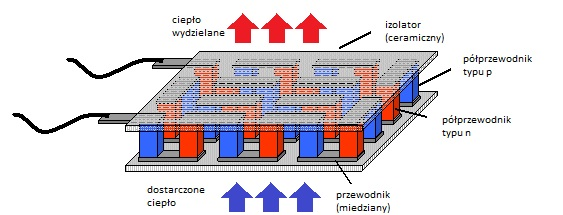
\includegraphics[scale=0.8]{budowaPeltier.jpg}
	\caption{Budowa modułu Peltiera}
\end{figure}
Półprzewodnikami wykorzystanymi do budowy ogniwa są tellurk oraz bizmut, które połączono ze sobą miedzianymi blaszkami. Istotą działania modułów Peltiera są zachodzące zmiany temperatur na połączeniach półprzewodników n-p, p-n, w wyniku przepływu prądu elektrycznego, którego wartość ma wpływ na ilość ciepła, które może zostać przetransportowana między stronami. Półprzewodnik typu n charakteryzuje się nadmiarową ilością elektronów, a typu p ich niewystarczalną ilością do wejścia na wyższy poziom energetyczny. Podczas przepływu prądu, elektrony przemieszczają się między poziomami energetycznymi, co w zależności od typu półprzewodnika oznacza zapotrzebowanie na dostarczenie energii (strona zimna) lub powoduje jej wydzielanie (strona ciepła). Niestety moduł nie jest idealny i część energii zostaje utracona w wyniku czego dochodzi również do ogrzania komponentów ogniwa.

Przydatną cechą modułów Peltiera jest możliwość połączenia ich kaskadowo tak by strona ciepła kolejnego ogniwa stykała się ze stroną zimną poprzedniego, co może pozwolić na wzrost wydajności układu. Ze względu na dużą ilość wydzielanego ciepła, zaleca się wykorzystanie pasty termoprzewodzącej oraz radiatorów po stronie ciepłej ogniwa.



\section{Arduino} %%jest OK
Arduino to sprzęt komputerowy i oprogramowanie stworzone przez firmę o tej samej nazwie, skupiające się na tworzenie zestawów uruchomieniowych opartych o mikrokontrolery z rodziny ATmega. Układ umieszczany jest na pojedynczej płytce drukowanej, z wyprowadzonymi wejściami i wyjściami układu. Język programowania  również nazywa się Arduino i został oparty o język C i C++. Najpopularniejszym ich produktem jest Arduino Uno. Wszystkie produkty wydawane są z otwartą licencją sprzętową i oprogramowania, dlatego na to na rynku dostępne są liczne klony płytek, zgodne z jej oryginalną specyfikacją. Urządzenia Arduino
może zostać wykorzystane jako samodzielny obiekt lub może być podłączone do komputera użytkownika.
\subsection{Hardware}%%jest OK
\begin{figure}[H]
	\centering
	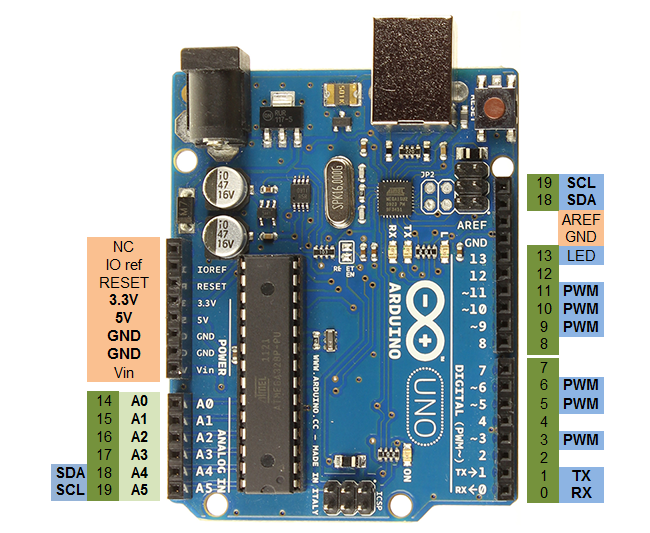
\includegraphics[scale=0.4]{ArduinoUno_pinout.png}
	\caption{Rozmieszczenie pinów dostępnych w Arduino Uno}
\end{figure}
Typowa płytka Arduino składa sie z mikrokontrolera, cyfrowych wejść/wyjść oraz wejść analogowych. Poza tym można na niej znaleźć takie interfejsy jak UART oraz USB do połączenia z komputerem, SPI i I2C do komunikacji z urządzeniami elektronicznymi.

W tej pracy wykorzystano płytkę Arduino Uno. Arduino Uno oparte jest o 8-bitowy mikrokontroler ATmega328, który uzupełniono elementami pozwalającymi na łatwiejsze programowanie wykorzystując port RS232 oraz sterowanie wyjściami mikrokontrolera. Płytka zawiera 5V regulator napięcia oraz rezonator kwarcowy o częstotliwości oscylacji 16MHz. Wyjścia mikrokontrolera zostały opisane i wyprowadzone jako żeńskie piny na obrzeżach płytki. Zastosowane rozwiązanie pozwala na łatwe podpięcie modułów rozszerzających funkcjonalność Arduino, nazywanych \textit{shieldami}. 

Arduino Uno posiada 6 wejść analogowych, 14 cyfrowych pinów wejścia/wyjścia, gdzie aż 6 z nich może zostać wykorzystane do generowania sygnału PWM. Oprócz tego można na niej znaleźć wyprowadzenia zasilania 3.3V i 5V. Piny analogowe zostały oznaczone literką A.
\newpage
\subsection{Programowanie}%%jest OK
\begin{figure}[H]
	\centering
	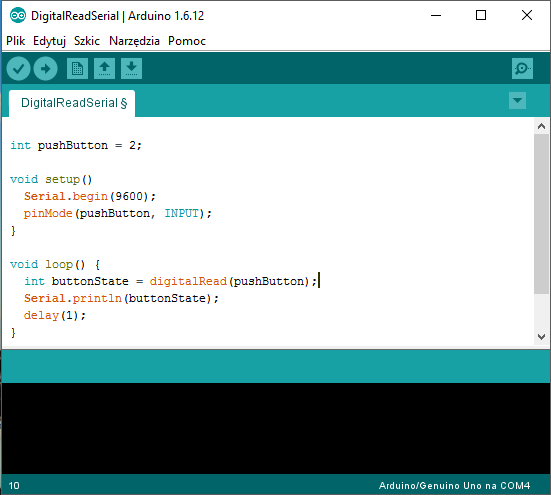
\includegraphics[scale=0.8]{arduinoIDE.png}
	\caption{Arduino IDE- przykładowy program}
	\label{ArduinoPodstawoweFunkcje}
\end{figure}
Do programowania płytek Arduino wykorzystuje się dedykowane oprogramowania Arduino IDE, które powstało na podstawie projektu Wiring oraz interfejs szeregowy RS232. Proces ten został ułatwiony poprzez wcześniejsze zaprogramowanie mikrokontrolera programem rozruchowym, zwalniającym z potrzeby używania zewnętrznego programatora. Oprogramowanie zawiera tak przydatne funkcje jak: kolorowanie składni kodu, automatyczne formatowanie, kompilację oraz wgrywanie programu na urządzenie docelowe. Zaletą Arduino IDE są dostępne opcje monitorowania portu szeregowego komputera w formie tekstowej, wykorzystując narzędzie ,,Monitor portu szeregowe'' oraz w postaci wykresu używając ,,Kreślarki''. Zawarta w programie biblioteka Wiring, będąca biblioteką C/C++, pozwala na ułatwienie wykonywania podstawowych operacji wejścia/wyjścia.

Aby stworzyć działający projekt należy zdefiniować dwie podstawowe funkcje:
\begin{itemize}
\item setup()- funkcja wykonywana tylko raz, wywoływana na początku programu w celu załadowania ustawień,
\item loop()- główne ciało programu, funkcja wykonywana jest wielokrotnie przez cały czas działania programu.
\end{itemize}


\section{Technologie internetowe}
\subsection{Cordova} %%jest OK
Apache Cordova to popularny framework służący do tworzenia aplikacji mobilnych w językach znanych deweloperom webowym. Cordova pozwala na utworzenie aplikacji na urządzenia mobilne wykorzystując HTML5, CSS3 oraz JavaScript. Jest to ciekawe rozwiązanie pozwalające na uniezależnienie się od środowisk programistycznych, specyficznych dla danej platformy jak np. Android Studio dla urządzeń z oprogramowaniem Android.

Cordova pozwala na napisanie jednej aplikacji, która następnie zostanie odpowiednio przetworzona, tak by działała na odpowiedniej platformie dystrybucji- urządzeniu Android lub iOS. W ten sposób uzyskuje się aplikację hybrydową, która nie jest w pełni natywna ze względu na interfejs użytkownika, który jest generowany w powłoce przeglądarki oraz nie w pełni webowa, bo zostaje skompilowana w paczkę dystrybucyjną, np. o rozszerzeniu app. Aplikacja ma dostęp do podzespołów telefonu, między innymi Bluetooth, WiFi, akcelerometr, GPS. 

\subsection{Ionic Framework}%%jest OK
Ionic to framework służący do tworzenia hybrydowych aplikacji mobilnych wykorzystujących HTML5, CSS i JavaScript. Został zbudowany z wykorzystaniem AngularJS oraz Apache Cordova. Takie rozwiązanie pozwala na dystrybucję aplikacji na różne platformy. Ionic mozna określić jako paczkę narzędzi, usług i stylów odpowiadającą za kreowanie przyjaznego interfejsu użytkownika. Jest ona odpowiednikiem wzbogaconego Bootstrapa w wersji dla aplikacji mobilnych.

Ionic zapewnia wszystkie funkcje dostępne w podstawowych SDK (zestaw narzędzi dla programistów, niezbędny w tworzeniu aplikacji na dany system) dla danej platformy. Interakcja z niestandardowymi komponentami i metodami udostępnionymi przez Ionic, możliwa jest poprzez wykorzystanie języka AngularJS.

\subsection{HTML}%%jest OK
HTML (HyperText Markup Language) to hipertekstowy język znaczników służący do tworzenia stron i aplikacji internetowych. W tej pracy wykorzystano HTML 5, który wywodzi się z języka HTML 4 i XHTML 1. Został on przyjęty za aktualny standard i jest wspierany przez wszystkie środowiska i producentów przeglądarek internetowych. Wraz z kaskadowymi arkuszami stylów i JavaScriptem tworzy on grupę najpopularniejszych technologii internetowych. HTML opisuje strukturę strony w sposób semantyczny, nadając treści dokumentu odpowiednie właściwości i funkcje, takie jak formowanie hiperłącza, list, nagłówków i akapitów. Do pozostałych funkcji tego języka należy możliwość załączania plików, plików graficznych i innych multimediów. Uzupełnieniem HTML jest CSS, który został opisany w kolejnym punkcie.

\subsection{Kaskadowe arkusze stylów}%%jest OK
Kaskadowe arkusze stylów (z ang. Cascading Style Sheets, w skrócie CSS) to język arkuszy stylów służący  do opisywania sposobu prezentacji zawartości dokumentu HTML, stron www. 
Arkusz stylów pozwala na opisanie wszystkich elementów dokumentu internetowego, takich jak: czcionka, kolor i rozmiar czcionki, interlinie, skalowanie elementów w zależności od rozmiarów otwartego okna oraz pozycjonowanie ich.

CSS został stworzony przez organizację W3C w 1996 roku w celu rozdzielenia warstwy prezentacji od warstwy danych. Uzyskane rozwiązanie pozwoliło na zwiększenie przejrzystości dokumentów HTML oraz ograniczyło ilość zmian wymaganych do wprowadzania podczas zmieniania stylu, który został wykorzystany na licznych podstronach.

\subsection{JavaScript}%%jest OK
JavaScript to dynamiczny, skryptowy język programowania wysokiego poziomu. Należy do grupy trzech najważniejszych języków, których musi się nauczyć każdy deweloper serwisów internetowych. Jest obsługiwany przez wszystkie nowoczesne przeglądarki internetowe bez potrzeby instalowania dodatkowych wtyczek. Mimo dużego podobieństwa w nazwie, języki Java i JavaScript znacznie różnią się składnią i dostępnymi bibliotekami. Język ten był wzorowany na C i przejął po nim między innymi funkcje warunkowe i pętle. W odróżnieniu od C jest to język prawie w pełni obiektowy.

Głównym zadaniem JavaScriptu jest zapewnienie interaktywności interfejsu użytkownika, czyli reakcja na wydarzenia takie jak wciśnięcie przycisku, wyświetlanie okien dialogowych, wywoływanie cyklicznych funkcji oraz aktualizowanie danych wyświetlanych na stronie. Poza tym pozwala na tworzenie ciasteczek i pobieranie informacji o przeglądarce użytkownika. JavaScript ma ograniczony dostęp do zasobów komputera użytkownika.

Do rozszerzenia funkcjonalności JavaScriptu wykorzystuje się lekkie biblioteki programistyczne takie jak jQuery, AngularJS ułatwiające manipulację obiektowym modelem dokumentu (z ang.DOM- Document Object Model), wykonywanie zapytań AJAX oraz dodawanie animacji na wyświetlanej stronie.

Skrypt JavaScript może zostać umieszczony na końcu dokumentu HTML, którego dotyczy, jednak ze względu na czytelność kodu i wymagany dostęp do niego dla wszystkich podstron, najczęściej zostaje umieszczony w osobnym pliku dodanym do projektu.

\subsection{AngularJS}%%jest OK
AngularJS to oparty na JavaScripcie, utworzony na otwartej licencji framework do tworzenia aplikacji internetowych, którego deweloperem jest Google. Głównym celem frameworka jest ułatwienie procesu deweloperskiego i testowania aplikacji poprzez wprowadzenie MVC (kontroler modelu widoku) po stronie użytkownika oraz MVVM (z ang. Model--viev--view-Model) w celu rozdzielenia kodu interfejsu od części logicznej.

AngularJS zaczyna pracę od przeszukania strony HTML w poszukiwaniu niestandardowych znaczników, które interpretuje i przypisuje do wejścia/wyjścia zmiennych wykorzystanych w JavaScipcie. Framework dopasowuje się do dokumentu HTML i rozszerza jego funkcjonalność o możliwość dynamicznego wyświetlania danych i aktualizowania widoku aplikacji, dzięki zaimplementowanemu dwukierunkowemu połączeniu między modelem i widokiem. Takie rozwiązanie pozwala znacznie ograniczyć ilość wymaganych do wykonania operacji w DOM.

Struktura programu w AngularJS składa się między innymi na zadeklarowany moduł aplikacji, kontroler i serwis.
\lstset{language=Java}
\begin{lstlisting} 
var app = angular.module('myApp', []);
app.controller('myController', function($scope) {
    $scope.firstName = "John";
    $scope.lastName = "Doe";
    $scope.personAge=myService.getAge();
})
app.service('myService', function() {
	var age=15;
    this.getAge = function () {
        return age;
    }
});
\end{lstlisting}
Zadaniem kontrolerów jest ingerowanie w interfejs użytkownika, reagowanie na wciśnięcia guzików oraz dokonywania zmian w wyświetlanych informacjach. \textit{Scope} to obiekt łączący ze sobą dane modelu i widoku. Serwisy tworzy się w celu zapewnienia funkcjonalności nie wpływającej bezpośrednio na interfejs, takiej jak np. pobieranie danych otrzymanych przez moduł Bluetooth, a następnie udostępnienie ich kontrolerowi poprzez funkcje zwracające wybrane dane.


\section{Komunikacja}
\subsection{Bluetooth}%%jest OK
Bluetooth to standard bezprzewodowej technologii wymiany danych na krótkim dystansie, pomiędzy urządzeniami typu klawiatura, komputer, bezprzewodowy głośnik, urządzenie mobilne, a w tym przypadku również Arduino. Został wymyślony przez firmę Ericsson w 1994 roku i został uznany za bezprzewodową alternatywę dla popularnego interfejsu RS232. Specyfikacja standardu Bluetooth obejmuje trzy klasy mocy nadawczej, 1-3 o zasięgu odpowiednio 100m, 10m i 1 metra w otwartej przestrzeni. W tej pracy wykorzystano moduł klasy 2, o zasięgu do 10 metrów.

Bluetooth pracuje na częstotliwości od 2402 do 2480 MHz, która jest globalnym standardem pasma częstotliwości krótkiego zasięgu dla zastosowań przemysłowych, naukowych i medycznych. Bluetooth dzieli wymieniane dane na pakiety. Każdy z nich zostaje wysłany na jeden z 79 wyznaczonych kanałów Bluetooth, których przepustowość wynosi 1 MHz. W przypadku modułów Bluetooth Low Energy o niższym poborze energii, kanałów jest jedynie 40, bo odstępy między nimi wynoszą aż 2 MHz. Protokół ten został oparty na strukturze Master-Slave. Zainicjować połączenie miedzy modułami może jedynie Master (w tym przypadku urządzenie mobilne), a Slave (moduł Bluetooth podłączony do Arduino) jedynie je zaakceptować. W tym protokole nie występuje problem z synchronizowaniem danych, dlatego że połączone ze sobą urządzenia otrzymują wspólny zegar, do którego działania zostaje dopasowany proces wysyłania i odbierania danych.

\subsection{UART}%%jest OK
UART ( z ang. Universal Asynchronous Receiver and Transmitter) to interfejs komunikacji szeregowej, szeroko wykorzystywany do przesyłania i odbierania danych asynchronicznie. Asynchroniczność oznacza, że dane są wysyłane nieregularnie. Ich początek i koniec jest oznaczony specjalnym symbolem. Interfejs UART został wykorzystany w tym projekcie do komunikacji między Arduino i modułem Bluetooth.
Procesor ATmega 328 znajdujący się na płytce Arduino Uno posiada specjalnie wyprowadzone piny portu szeregowego:
\begin{itemize}
\item{RXD- wejście szeregowe (,,Receive Data''),}
\item{TXD- wyjście szeregowe (,,Transmit Data'').}
\end{itemize}
Zaletą interfejsu UART jest posiadany przez niego bufor danych przeznaczony do tymczasowego przechowywania informacji w sytuacji, gdy są one szybko transmitowane.
Ten rodzaj transmisji danych charakteryzuje się również tym, że nadajnik i odbiornik nie posiada wspólnego sygnału zegarowego. W tym przypadku każde z urządzeń działa w takt własnego zegara. Podczas połączenia urządzeń należy pamiętać, aby oba miały ustawioną taką samą częstotliwość taktowania zegara.

\subsection{1-Wire}%%jest OK
One Wire to systemowa magistrala komunikacji elektronicznej pomiędzy urządzeniami, zapewniająca przesyłanie danych oraz zasilanie urządzenia przez pojedynczy kabel. Proces ten jest możliwy dzięki stopniowemu ładowaniu kondensatora znajdującego się w odbiorniku, a następnie wykorzystanie zgromadzonej energii do zasilenia urządzenia. Do magistrali może zostać podłączonych wiele urządzeń. Każdemu z nich przydzielany jest indywidualny adres 64-bitowy. Komunikację z urządzeniami inicjuje master, w tym przypadku mikrokontroler.

Przedstawiony protokół jest bardzo podobny do I2C, ale ze względu na wykorzystanie jedynie jednej linii danych, charakteryzuje się niższą prędkością przesyłania. Układ zazwyczaj zasilany jest napięciem o wartości 5V i służy do komunikacji pomiędzy niewielkimi urządzeniami, takimi jak np. termometr cyfrowy i mikrokontroler.



%%%%%%%%%%%%%%%%%%%%%%%%	Część konstrukcyjna  \\\\\\wygląda ok \\ZMIEN ZDJECIA
\chapter{Konstrukcja obiektu i układu regulacji}
Główne założenia dotyczące tej pracy zostały przedstawione w drugim rozdziale tego raportu. W tym rozdziale przedstawiono konstrukcję obiektu regulacji temperatury oraz połączenie komponentów elektrycznych w funkcjonalną całość.

Celem tej pracy było stworzenie układu pomiarowo-regulacyjnego. Główną jednostką operacyjną jest płytka Arduino, pełniąca rolę sterownika kontrolującego wszystkie podzespoły oraz odpowiedzialnego za udostępnianie danych urządzeniom mobilnym.


\section{Wykorzystane podzespoły} 
W tym rozdziale przedstawiono podstawowe informację na temat najważniejszych wykorzystanych peryferiów.
\subsection{LCD}%%jest OK
\begin{figure}[H]
	\centering
	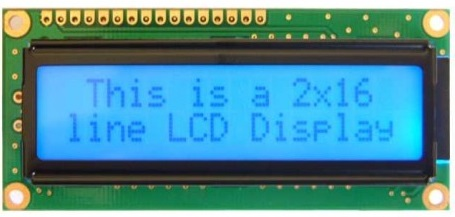
\includegraphics[scale=0.8]{lcd2x16.jpg}
	\caption{Ekran LCD 2x16 znaków}
\end{figure}
Do wyświetlania danych wybrano popularny wyświetlacz LCD 2x16 znaków, ze sterownikiem HD44780, odpowiedzialnym za wyświetlanie odebranych danych. Moduł zasilany jest napięciem 5V i może być sterowany w 4 trybach:
\begin{itemize}
\item 8-bitowym bez odczytu flagi zajętości,
\item 8-bitowym z odczytem flagi zajętości,
\item 4-bitowym z odczytem flagi zajętości,
\item 4-bitowym bez odczytu flagi zajętości.
\end{itemize}
Ze względu na ograniczoną ilość pinów Arduino zdecydowano się na wykorzystanie ostatniego z wymienionych trybów.

 \begin{table}[H]
	\centering
	\caption{Opis pinów ekranu LCD}
	\begin{tabular}{|c|c|c|}
		
  \hline 
  \bfseries Nr & \bfseries Nazwa & \bfseries Opis \\
  \hline
  1&VSS&Masa  \\
  \hline
  3&V0&Kontrast  \\
  \hline
  4&RS&Wybór rejestru instrukcji wyświetlacza (stan niski)\\
   &&albo rejestru danych (wysoki) \\
  \hline
  5&R/W& Odczyt (stan niski)/ Zapis (stan wysoki)  \\
  \hline
    6&E& Odblokowanie wyświetlacza  \\
  \hline
      7-14&DB0-7& Magistrala danych  \\
  \hline
        15&LEDA& Zasilanie podświetlania +5V  \\
  \hline
        16&LEDK& Masa podświetlenia  \\
  \hline
\end{tabular}
\end{table}

\subsection{DS18B20}
DS18B20 to popularny termometr cyfrowy wyposażony w interfejs komunikacyjny 1-wire. Podjęto decyzję o wykorzystaniu tego komponentu, dlatego że oferował on wystarczająco dużą dokładność pomiarową i możliwość poznania wcześniej nieznanego autorowi protokołu komunikacyjnym.
\begin{figure}[H]
	\centering
	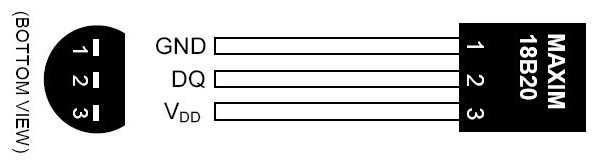
\includegraphics[scale=0.65]{ds18b20.jpg}
	\caption{Opis wyprowadzeń czujnika temperatury DS18B20}
\end{figure}
Termometr cyfrowy DS18B20 posiada jedynie trzy wyprowadzenia:
\begin{itemize}
\item VDD- napięcie zasilania mogące wynosić od 3V do 5,5V,
\item DQ- sygnał cyfrowy,
\item GND- masa układu.
\end{itemize}
Przedstawiony termometr pozwala na mierzenie temperatury w zakresie $-55^{\circ} C$ do $125^{\circ} C$. Rozdzielczość termometru może zostać dostosowana przez użytkownika, poprzez wybranie ilości otrzymywanych bitów danych. Istnieje możliwość wyboru trybu 9, 10, 11, 12 bitowego, odpowiadającego wartościom 0.5, 0.25, 0.125 i 0.625 stopnia Celsjusza. Zdecydowano się na wybór trybu 12 bitowego, w celu poprawy działania regulatora. Na wyświetlaczu oraz urządzeniu mobilnym wartość została zaokrąglona do jednego miejsca po przecinku.
%\subsection{Termometr LM35}%%jest OK
%\begin{figure}[H]
%	\centering
%	\includegraphics[scale=0.5]{lm35.jpg}
%	\caption{Termometr LM35}
%\end{figure}
%LM35DZ to analogowy czujnik temperatury, którego wyjście przyjmuje wartość napięcia proporcjonalną do zmierzonej temperatury. Termometr działa w zakresie temperatur od 90 do 100 stopni Celsjusza. Czujnik został fabrycznie skalibrowany do mierzenia temperatury w stopniach Celsjusza. Dokładność pomiaru wynosi około 0,5 C.
%
%Termometr cyfrowy LM35 posiada jedynie trzy wyprowadzenia:
%\begin{itemize}
%\item VDD- napięcie zasilania mogące wynosić od 4V do 30V
%\item OUT- sygnał analogowy,
%\item GND- masa układu.
%\end{itemize}
\subsection{Moduł Bluetooth HC-06}%%jest OK

W fazie powstawania pierwotnej koncepcji projektu zastanawiano się nad wyborem sposobu komunikacji bezprzewodowej między mikrokontrolorem, a urządzeniem mobilnym z oprogramowaniem Android. Rozważanymi technologiami był moduł XBee oraz moduł Bluetooth. Ze względu na cenę modułów oraz wymaganą ilość wejść/wyjść mikrokontrolera zdecydowano się na zakup modułu Bluetooth HC-06, pozwalającego na pracę pinów danych w logice 5V..
\begin{figure}[H]
	\centering
	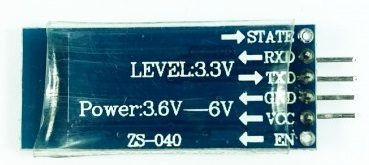
\includegraphics[scale=0.5]{hc06.jpg}
	\caption{Moduł Bluetooth HC-06}
\end{figure}
Charakterystycznymi cechami wybranego modułu jest zasięg do około 10m i fabrycznie ustawiony tryb slave, bez możliwości przejścia w tryb master (inicjacja połączenia między modułami), którym w tym przypadku jest telefon komórkowy lub tablet. Moduł przekazuje dane z prędkością 9600 bitów na sekundę.

\begin{table}[H]
	\centering
	\caption{Opis wejść/wyjść modułu Bluetooth HC-06}
	\begin{tabular}{|c|c|c|}
		
  \hline 
 \bfseries Nr & \bfseries Nazwa & \bfseries Opis \\
  \hline
  1&STATE& Informacja o połączeniu z innym urządzeniem  \\
  \hline
  2&RXD& Komunikacja szeregowa  \\
  \hline
  3&TXD& Komunikacja szeregowa \\
  \hline
  4&GND& Masa układu \\
  \hline
    5&VCC& Zasilanie  \\
  \hline
      6&EN&Pin pozwalający na włączenie trybu konfiguracji modułu \\
  \hline
\end{tabular}
\end{table}
\subsection{L293D}%%jest OK
\begin{figure}[H]
	\centering
	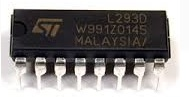
\includegraphics[scale=0.65]{l293d.jpg}
	\caption{Sterownik silników L293D}
\end{figure}
L293D to dwukanałowy sterownik silników o napięciu zasilania do 36V. Moduł zazwyczaj określany jest jako mostek H, ale w rzeczywistości składa się z czterech połowicznych mostków H. Charakteryzują się one tym, że posiadają tylko dwa tranzystory po jednej stronie obciążenia. Sterownik pozwala na zasilenie urządzenia o średnim poborze prądu o wartości 0,6A, a nawet do 1,2A w przypadku pracy krótkotrwałej. Moduł chroniony jest przez obudowę DIP z wyprowadzonymi 16 nóżkami. Moduł został wykorzystany do sterowania dwoma silnikami DC o napięciu znamionowym 12V.
\begin{table}[H]
	\centering
	\caption{Opis wejść/wyjść L293D}
	\begin{tabular}{|c|c|c|}
		
  \hline 
 \bfseries Nr & \bfseries Nazwa & \bfseries Opis \\
  \hline
    1&ENABLE1&Sygnał sterujący(PWM) kanału pierwszego \\
  \hline
      2,7&INPUT1-2&Kierunek kanału pierwszego  \\
  \hline
  3,6&OUTPUT1-2&Wyjście kanału pierwszego  \\
  \hline
           8&VS&Zasilanie silników  \\
  \hline
    9&ENABLE2&Sygnał sterujący(PWM) kanału drugiego \\
  \hline
       10,15&INPUT3-4&Kierunek kanału drugiego  \\
  \hline
  11,14&OUTPUT3-4&Wyjście kanału drugiego  \\
  \hline
       16&VSS&Zasilanie części logicznej  \\
  \hline
           4,5,12,13&GND&Masa układu  \\
  \hline
\end{tabular}
\end{table}
\newpage
\subsection{DFRobot - dwukanałowy sterownik silników }%%jest OK

\begin{figure}[H]
	\centering
	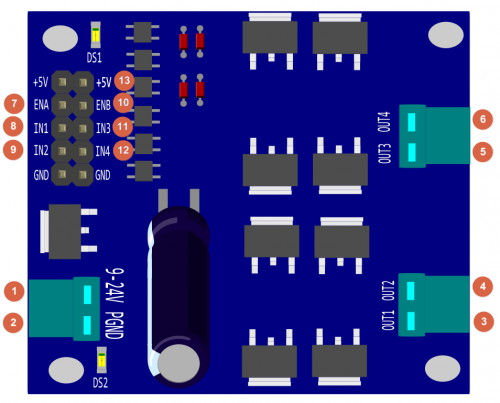
\includegraphics[scale=0.5]{dfrobot.jpg}
	\caption{Sterownik silników DFRobot}
\end{figure}
Moduł DFRobot to dwukanałowy sterownik silników prądu stałego. Urządzenie powinno zostać zasilone napięciem od 6,5 do 27V. Pozwala na zasilenie silnika o średnim poborze prądu do 7 A, a w przypadku wartości chwilowych aż do 50 A. Sterownik ten został wybrany ze względu na dużą moc i dwukanałowość, która mogłaby okazać się potrzebna w sytuacji gdy jedno ogniwo byłby za słabe by znacznie wpływać na temperaturę w obiekcie. Układ pracuje w logice 3,3 V oraz 5V. Sterowanie modułem przebiega w ten sam sposób jak w przypadku sterownika L293D, na dwa piny sterujące podajemy odpowiednią kombinację 0 i 1 logicznej, tym samym wyznaczając kierunek obrotów, a następnie na kolejnym pinie zadajemy prędkość wykorzystując sygnał PWM.
\begin{table}[H]
	\centering
	\caption{Opis wejść/wyjść sterownika DFRobot}
	\begin{tabular}{|c|c|c|}
		
  \hline 
  \bfseries Nr & \bfseries Nazwa & \bfseries Opis \\
  \hline
    1&9-24V&Napięcie zasilania \\
  \hline
     2&IPGND&Masa układu  \\
  \hline
  3,4&OUT1/2&Wyjście 1/2 kanału A  \\
  \hline
           5,6&OUT3/4&Wyjście 1/2 kanału B  \\
  \hline
    7&ENA&PWM dla kanału A \\
  \hline
       8,9&IN1/2&Wejście sterujące 1/2 kanału A  \\
  \hline
  10&ENB&PWM dla kanału B  \\
  \hline
       11,12&IN3/4&Wejście sterujące 1/2 kanału B  \\
  \hline
           13&+5V&Napięcie referencyjne: 3,3V lub 5V  \\
  \hline
\end{tabular}
\end{table}
\subsection{Ogniwo Peltiera TEC-12706}%%jest OK
Ogniwo Peltiera zostało szerzej opisane na we wstępie teoretycznym do pracy. W opisanym projekcie użyto ogniwa Peltiera zasilanego napięciem 12V (do 15V) oraz o średnim poborze prądu wynoszącym 4,5A (maksymalnym 6A).
\begin{figure}[H]
	\centering
	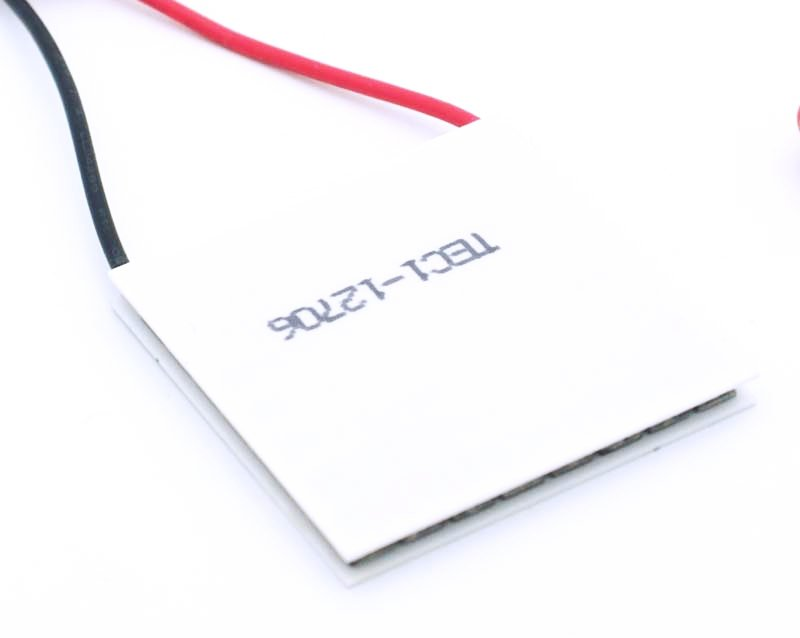
\includegraphics[scale=0.15]{tec12706.jpg}
	\caption{Moduł ogniwa Peltiera (wym. 40x40x3,8 mm)}
\end{figure}
Ogniwo to charakteryzuje się maksymalną mocą wejściową około 90W i mocą odprowadzania ciepła do 53,3W. Sprawność ogniwa zależy od szczelności termicznej chłodzonego/ogrzewanego obiektu. Zdecydowano się na wybór takiego ogniwa ze względu na łatwo dostępne źródło zasilania, pozwalające na osiągnięcie maksymalnej mocy ogniwa. Jest to wersja ogniwa najczęściej wykorzystywana w lodówkach turystycznych, popularna ze względu na możliwość zasilenia przez gniazdko zapalniczki samochodowej.

\subsection{Wiatrak komputerowy- silnik DC}%%jest OK
Ze względu na szeroki zakres dostępu do starych komponentów komputerowych wybrano wiatraki wykorzystywane do chłodzenia procesorów. Silnik charakteryzuje się napięciem znamionowym 12V i poborem prądu o wartości 0,6A. W początkowej fazie projektu używano wiatraka promieniowego, ale ze względu na duży hałas podczas pracy podjęto decyzje o wymianie na wiatrak komputerowy. Silnik może obracać się z prędkością od 2500 do 3400 obrotów na minutę.
\begin{figure}[H]
	\centering
	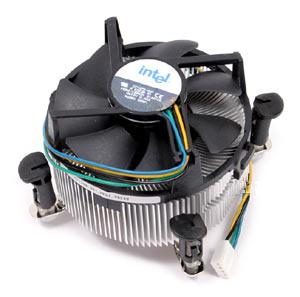
\includegraphics[scale=0.6]{wiatrakDC.jpg}
	\caption{Wykorzystany wiatrak (bez radiatora)}
\end{figure}
Każdy z wiatraków posiada 3 piny:
\begin{itemize}
\item 1- napięcie zasilania silnika,
\item 2- uziemienie układu,
\item 3- sygnał z halotronu.
\end{itemize}

\subsection{Zasilacz ATX}
Do zasilenia układu wykorzystano zasilacz ATX firmy MODECOM o mocy 350W. Układ został wykorzystany ze względu na fakt, że był dostępny po rozebraniu na części starego komputera stacjonarnego autora. Dodatkową zaletą okazały się wyprowadzenia zasilania na 5 V, użyte do uruchomienia Arduino oraz wyjścia 12 V, wykorzystane do zasilenia wiatraków i ogniwa Peltiera.
\begin{figure}[H]
	\centering
	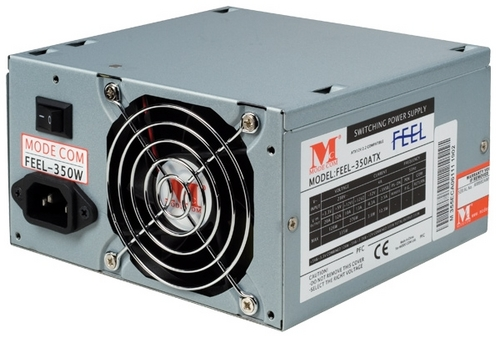
\includegraphics[scale=0.4]{modecom.jpg}
	\caption{Zasilacz ATX}
\end{figure}
\section{Obiekt pomiarowy}%%jest OK
\begin{figure}[H]
	\centering
	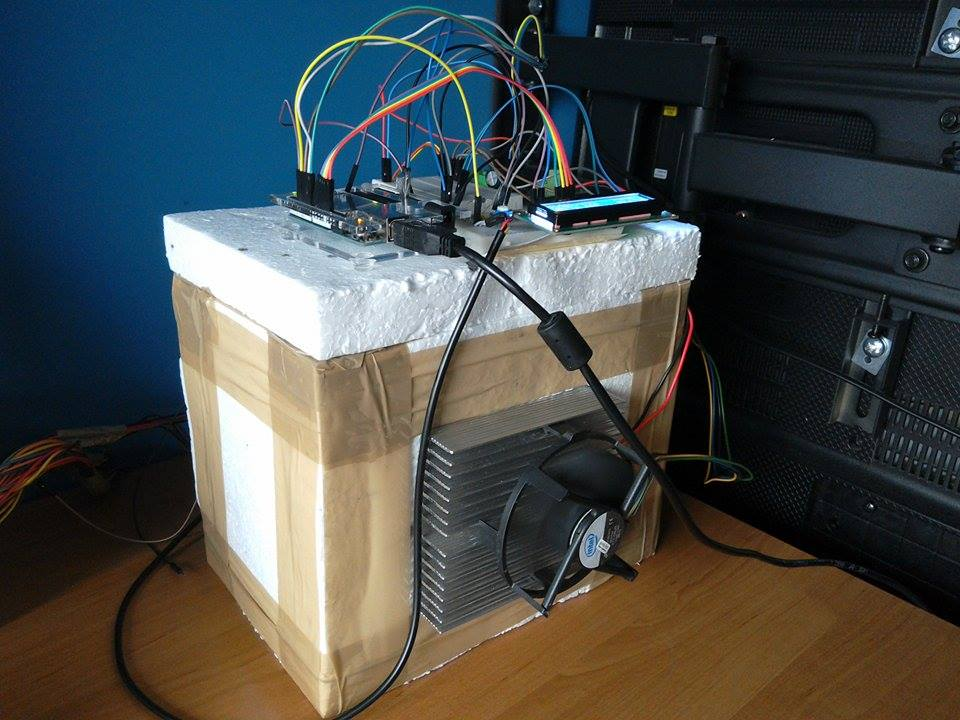
\includegraphics[scale=0.25]{stanowisko.jpg}
	\caption{Obiekt regulacji temperatury}
\end{figure}
Podczas konstruowania obiektu pomiarowego za najważniejsze czynniki konstrukcyjne przyjęto: izolację termiczną materiału z którego zostanie wykonany, łatwość modelowania go oraz koszty wykorzystania. Dlatego zdecydowano się na styropian do ocieplania fasad. Cechy te okazały się bardzo korzystne ze względu na fakt, że rozmiar i wygląd "pomieszczenia" był kilkukrotnie modyfikowany z powodów takich jak zbyt słabe uszczelnienie czy też zbyt duży rozmiar obiektu niepozwalający na znaczny wpływ ogniwa Peltiera na temperaturę w obiekcie w rozsądnym przedziale czasowym. Ostateczna konstrukcja przyjęła postać styropianowego prostopadłościanu.

Kolejną częścią, która wymagała przemyślenia było miejsce i sposób zamontowania ogniwa Peltiera, tak by mogło ono optymalnie chłodzić i ogrzewać pomieszczenie. Ogniwo zostało zamontowane na bocznej ścianie. Dodatkowym powodem przemawiającym za takim rozwiązaniem było wolne miejsce na dachu, w którym zamontowano Arduino i pozostałe podzespoły.

Ze względu na dużą ilość wydzielanego ciepła ze strony ciepłej podczas chłodzenia obiektu, ogniwo musiało zostać przymocowane do dużych radiatorów z obu stron. Do części ogniwa bezpośrednio wpływającej na wnętrze obiektu przymocowano najpierw aluminiowy blok, a następnie radiator. Takie rozwiązanie zastosowano w celu ograniczenia wpływu temperatury radiatora znajdującego się na zewnątrz na część wewnętrzną. 

Jednak nawet takie rozwiązanie okazało się nie być pozbawione wad. Przy długotrwałym chłodzeniu obiektu, strona gorąca nagrzewała się tak bardzo, że różnica temperatury pomiędzy dwoma stronami ogniwa była zbyt duża, co powodowało stopniowe nagrzewanie się strony chłodzącej. Sytuacja taka wynika z tego, że różnica temperatur między stroną ciepłą a zimną ma swoją wartość maksymalną, po przekroczeniu której dochodzi do ogrzania części chłodnej, w celu zmniejszenia różnicy temperatur. 
Skutecznym rozwiązaniem tego problemu okazało się dołączenie wiatraczka komputerowego do każdego z radiatorów. Zabieg ten poprawił prędkość oddawania temperatury do powietrza oraz jego cyrkulację w obiekcie, w wyniku czego procesy regulacji temperatury stały się dynamiczniejsze. Ostatnim elementem konstrukcji jest termometr, który został wprowadzony do środka obiektu poprzez jedną z bocznych ścian.

\section{Układ wykonawczy}
Główną jednostką obliczeniową układu jest Arduino, do którego zostały podłączone podzespoły składające się na:
\begin{itemize}
\item sterownik silników DFRobot,
\item ogniwo Peltiera,
\item dwukanałowy sterownik silników L293D,
\item 2 silniki DC,
\item ekran LCD 2x16,
\item termometr analogiczny LM35,
\item moduł Bluetooth HC-06,
\end{itemize}
których obsługa została szerzej opisana w kolejnym rozdziale.
Do podłączenia układu wykorzystano 800 stykową płytkę prototypową, na której umieszczono ekran LCD i pozostałe mieszczące się moduły. Komponenty zostały połączone zgodnie z opisami pinów i zaleceniami zawartymi w dokumentacji producentów. Na poniższym rysunku można zobaczyć schemat połączeń urządzeń.

\begin{figure}[H]
	\centering
	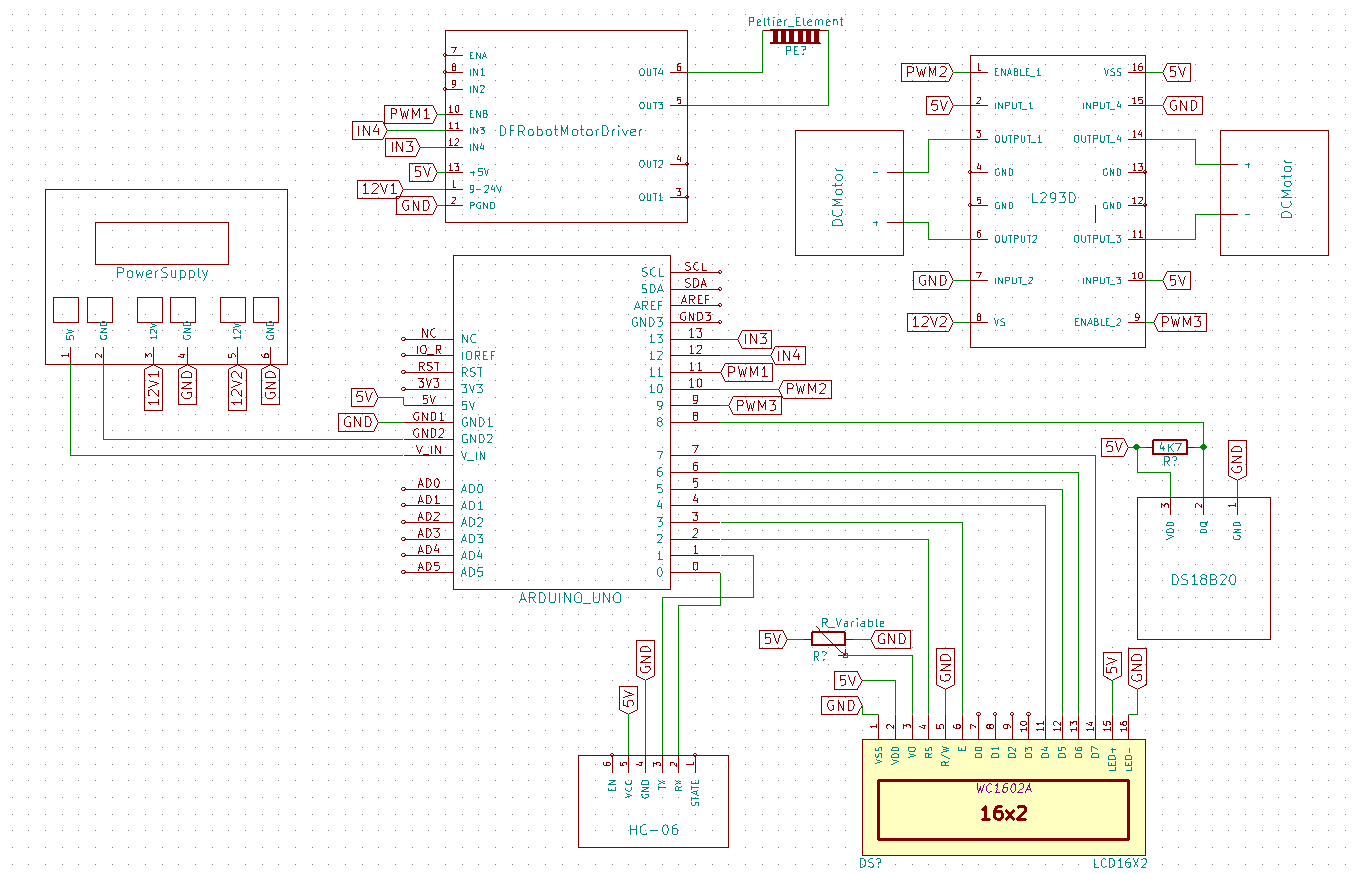
\includegraphics[scale=0.4]{schemat.png}
	\caption{Schemat połączeń elektrycznych}
\end{figure}



%%%%%%%%%%%%%%%%%%%%%%%%	Arduino \\\w trakcie
\chapter{Sterowanie układem regulacji temperatury- Arduino}
\section{Główna pętla programu} %OK
\begin{figure}[H]
	\centering
	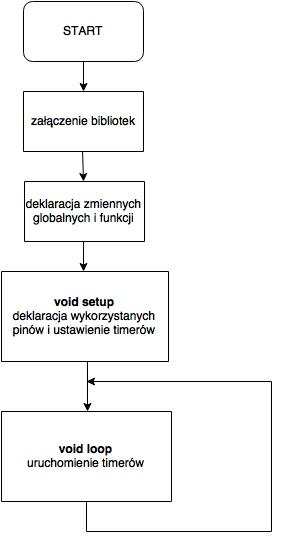
\includegraphics[scale=0.65]{mainProgram.jpg}
	\caption{Główna pętla programu}
\end{figure}
Struktura programu napisanego w języku Arduino przypomina strukturę charakterystyczną dla języka C/C++. Na początku pliku zadeklarowane zostają wykorzystane biblioteki. W tym przypadku użyto trzech:
\begin{itemize}
\item \textit{Simple Time}- tworzenie niestandardowych timerów,
\item \textit{Liquid Crystal}- obsługa wyświetlacza LCD,
\item \textit{OneWire}- odczyt danych z urządzeń korzystających z technologii OneWire.
\end{itemize}
Następnie utworzone zostają zmienne globalne, dostępne dla wszystkich funkcji. 
Przechowują one wartości nastaw regulatorów, aktualne odczyty oraz numery wykorzystanych wejść/wyjść mikrokontrolera. Następnie zostają zdefiniowane funkcje utworzone w programie.

Program składa się na dwie główne części opisane i zaprezentowane na Rysunku nr. \ref{ArduinoPodstawoweFunkcje}. W wykonywanej tylko raz funkcji \textit{void setup(void)} piny Arduino zostały ustawione jako wyjścia lub wejścia. Wejściem został jedynie pin nr. 8 podłączony do termometru. Wywołana została funkcja \textit{setLCD\_start()}, odpowiadająca za wyświetlenie na ekranie informacji, których odświeżanie nie będzie konieczna. Ostatnią rzeczą wykonaną na tym etapie jest utworzenie nowych timerów odpowiadających za:
\begin{itemize}
\item regulację temperatury co 1 sekundę,
\item wysyłanie danych co 1 sekundę,
\item odbieranie danych co 2 sekundy.
\end{itemize}

W nieustannie wykonywanej funkcji \textit{void loop(void)} zadano silnikom pracę z maksymalną prędkością obrotową. Została wykonana metoda \textit{timer.run} uruchamiająca pracę wcześniej utworzonych timerów.

W kolejnych sekcjach opisano działanie funkcji wywoływanych przez timery oraz obsługę urządzeń peryferyjnych.

\section{Odbiór danych}%OK
Do komunikacji między urządzeniami wykorzystano moduł Bluetooth, połączony z Arduino przez port szeregowy UART. Do obierania danych przesłanych przez urządzenie mobilne utworzono funkcję \textit{bluetoothReceive()}, wywoływaną przez timer co 2 sekundy. Wejście RX Arduino zostało połączone z wyjściem TX modułu. Pozostałe piny połączono adekwatnie. Komunikacja odbywa się poprzez przesłanie ramki danych o wyznaczonym symbolu rozpoczęcia i zakończenia ciągu danych. Struktura ramki została przedstawiona na rysunku \ref{ramka1}.
\begin{figure}[H]
\centering
\Huge "tXpXjXdXrXhXmX/n"
\label{ramka1}
\caption{Ramka komunikacji od urządzenia mobilnego do Arduino}
\end{figure}
Znaki \textit{X} oznaczają wartości parametrów. Przez małe litery oznaczono informację o początku danego parametru:
\begin{itemize}
\item \textit{t}- temperatura zadana,
\item \textit{p}- wzmocnienie części proporcjonalnej,
\item \textit{i}- wzmocnienie części inercyjnej,
\item \textit{d}- wzmocnienie części różniczkującej,
\item \textit{r}- typ regulatora, PID lub histerezowy,
\item \textit{h}- wartość histerezy,
\item \textit{m}- moc regulatora histerezowego,
\item \textit{/n}- zakończenie ramki.
\end{itemize}
Na początku działania funkcji odbioru danych zostają utworzone zmienne dla każdego określonego znaku charakterystycznego i parametru. W celu ułatwienia konwersji danych, dla parametrów utworzono zmienne typu string oraz int lub float.

Przed rozpoczęciem pobierania wykonane zostaje polecenie sprawdzające czy bufor portu szeregowego przechowuje jakieś dane. Jeśli tak, to zostaje wykonane polecenie \\ \textit{Serial.readStringUntil('/n')}, zapisujące wszystkie znaki przechowywane przez bufor, aż do napotkania znaku zakończenia ramki ,,/n''. Jeśli długość otrzymanego ciągu znaków jest równa lub większa od minimalnej długości ramki, to rozpoczyna się proces obróbki danych.

Kolejnym krokiem jest wykonanie się pętli \textit{for}, której zadaniem jest znalezienie wszystkich określonych znaków charakterystycznych i przypisanie ich położenia w ciągu znaków do zmiennej o tym samym symbolu co znak, którego położenie określa.

Następnie za pomocą polecenia \textit{String.substring(a,b)} z otrzymanego ciągu znaków zostają wycięte części odpowiadające wartościom parametrów, które zostają zapisane do zmiennych string. Aby zamienić ciągi znaków na liczby, użyto metod \textit{String.toInt()} oraz \textit{String.toFloat}. Powstałe wartości liczbowe przypisano do zmiennych globalnych.
\newpage
\section{Regulacja temperatury}%jest ok
\begin{figure}[H]
	\centering
	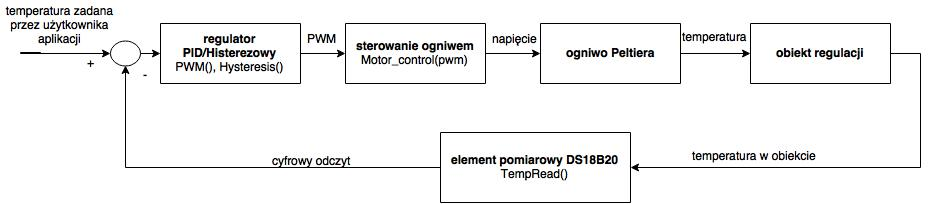
\includegraphics[scale=0.45]{regulacjatemp.jpg}
	\caption{Schemat regulacji temperatury}
\end{figure}
Funkcja \textit{void regulation()} wywoływana przez drugi timer jest odpowiedzialna za proces regulacji temperatury, na który składa się: odczyt aktualnej wartości temperatury, obliczenie sygnału sterującego PWM oraz sterowanie ogniwem za pomocą funkcji przedstawionych na poniższym listingu.
\lstset{language=C++}
\lstset{
	basicstyle=\footnotesize,
	breaklines=true,
	showspaces=false,
	%inputencoding=utf8, 
	%extendedchars=\true,
	literate={ą}{{\k{a}}}1
             {Ą}{{\k{A}}}1
             {ę}{{\k{e}}}1
             {Ę}{{\k{E}}}1
             {ó}{{\'o}}1
             {Ó}{{\'O}}1
             {ś}{{\'s}}1
             {Ś}{{\'S}}1
             {ł}{{\l{}}}1
             {Ł}{{\L{}}}1
             {ż}{{\.z}}1
             {Ż}{{\.Z}}1
             {ź}{{\'z}}1
             {Ź}{{\'Z}}1
             {ć}{{\'c}}1
             {Ć}{{\'C}}1
             {ń}{{\'n}}1
             {Ń}{{\'N}}1
	}
\begin{lstlisting}
void regulation() {
  temperatureReading = TempRead();	//odczyt temperatury
  if (regulatorType == 0) {	
    pwm = PID(temperatureSetpoint, temperatureReading, millis(), kp , ki, kd); //wywołanie własnego regulatora PID
  }
  else {	//wywołanie regulatora histerezowego
    pwm = HIST(temperatureSetpoint, temperatureReading, hysteresis, power);
  }
  Motor_Control(pwm);	//funkcja sterująca ogniwem
}
\end{lstlisting}
Proces rozpoczyna się od wywołania funkcji odczytującej temperaturę. Następnie zostaje sprawdzony typ regulatora zapisany w postaci cyfry. W zależności od wyboru użytkownika, zostaje użyty regulator histerezowy lub PID. Wartości parametrów każdego z nich mogą zostać dostosowane w aplikacji mobilnej. Otrzymany sygnał sterujący zostaje przekazany funkcji sterującej ogniwem.
\subsection{Odczyt temperatury}
Do odczytu temperatury zmierzonej przez termometr cyfrowy DS18B20 użyto biblioteki \textit{OneWire} oraz funkcji dedykowanej dla wybranego termometru, dostępnej na stronie producenta Arduino. Na początku programu utworzono obiekt \textit{OneWire ds(8)}, któremu zostało przypisane ósme wejście mikrokontrolera.

Funkcja rozpoczyna swoje działanie od wyszukania urządzeń podłączonych do linii OneWire. Znaleziony adres zostaje przechowany w zmiennej. Następnie za pomocą polecenia \textit{ds.select(addr)}, zostaje nawiązana komunikacja z wybranym urządzeniem. W kolejnym etapie do termometru zostaje wysłane wymuszenie odczytu danych. Termometr zapisuje do \textit{brudnopisu} wartość uzyskaną od wbudowanego przetwornika analogowo-cyfrowego. Dane przechowywane w \textit{brudnopisie} mogą zostać odczytane w każdej chwili. Jeśli nie zostało wcześniej wykonane polecenie konwersji, to termometr zwróci ostatnią odczytaną wartość. Czas trwania konwersji danych zależy od rozdzielczości, jaką chce osiągnąć użytkownik. Do termometru zostaje przesłana wartość \textit{0xBE}, w odpowiedzi na którą urządzenie udostępnia pomiar. W celu uzyskania największej rozdzielczości, należy odczytać 12 bitów danych, które następnie zostają zamienione na pomiar temperatury.

\subsection{Regulator PID} %to ok
Regulator PID zbudowany jest z 3 członów: proporcjonalnego (P), inercyjnego (I) i różniczkującego (D). Zaimplementowany regulator posiada funkcję anti-windup. Najważniejszymi argumentami funkcji są: aktualna temperatura, wartość zadana oraz parametry. Język Arduino nie posiada zaimplementowanego działania całkowania ani różniczkowania, dlatego działania te musiały zostać uproszczone. Użyto całkowania i różniczkowania numerycznego. Regulacja wykonywana jest przez układ dyskretny.

\begin{lstlisting} 
int PID(int setpointTemperature, float currentTemperature, float actualTime, int kp, int ki, int kd) {
  float maximum = 255;
  float minimum = -255;
  float static integral = 0;
  float static previousTime = 0;
  float static previousError = 0;
  float static previousOutput=0;
  float error = setpointTemperature - currentTemperature;
  float dt = (float)(actualTime - previousTime);
  dt=dt/60000; //przeskalowanie czasu na minuty
  if(previousOutput>-255&&previousOutput<255){	//anty-windup
    integral = integral + (error * dt);	//człon całkujący
  }
  if (integral > 1) {	//ograniczenie całki
    integral = 1;
  }
  else if (integral < -1) {
    integral = -1;
  }
  float derivative = (error - previousError) / dt;	//człon różniczkujący
  previousError = error;
  previousTime = actualTime;
  int output = kp * error + ki*integral + kd * derivative; //sygnał wyjściowy
  previousOutput=output;
  if (output >= maximum){	//ograniczenie wartości wyjścia
    output = maximum;
  }
  else if ( output <= minimum){
    output = minimum;
  }
  return output;
}
\end{lstlisting}
Na potrzeby prawidłowego działania regulatora, utworzono zmienne określające maksymalne wartości wyjścia regulatora oraz zmienne statyczne, przechowujące dane potrzebne w kolejnych wywołaniach funkcji. Na początku zostaje obliczony błąd regulacji- \textit{error} oraz czas- \textit{dt} jaki upłynął od poprzedniego wywołania funkcji. Uzyskana wartość czasu zostaje przeskalowana do minut. Następnie sprawdzone zostaje jaką wartość przyjęła poprzednia instancja regulatora. Jeśli mieści się ona w zakresie od -255 do 255, to zostaje obliczona nowa wartość części inercyjnej regulatora. Takie rozwiązanie zostało potraktowane jako zaimplementowanie systemu anty-windup. Dzięki tej funkcji, człon całkujący nie będzie dalej narastał, gdy wyjście ma wartość maksymalną. Dodatkowo nałożono ograniczenie wartości maksymalnej członu całkującego. Wartość całki została uproszczona do sumy poprzedniej wartości całki i błędu pomnożonego przez czas \textit{dt}. W kolejnym kroku, sprawdzane jest, czy wartość całki mieści się w określonym zakresie. W przypadku niespełnienia warunku, całka zostaje ograniczona.Człon różniczkujący został obliczony przez różnicę aktualnego błędu regulacji i poprzedniego błędu podzielonego przez \textit{dt}. Sposób zapisu uproszczonych działań wzorowany jest na źródle [1] oraz przykładzie, który przedstawiono podczas zajęć dydaktycznych. Wartość błędu i aktualny czas zostają zapisane do zmiennych statycznych.

Wyjście regulatora zostaje wyznaczone przez pomnożenie obliczonych członów przez odpowiadające im wzmocnienia, które następnie zostają zsumowane. Wyjście regulatora zostaje ograniczone do przedziału od -255 do 255, w celu nieprzekroczenia maksymalnej wartości sygnału PWM.

\subsection{Regulator histerezowy}%jest ok
Regulacja histerezowa polega na regulowaniu temperatury poprzez ustalenie zakresów, dla których obiekt grzewczy będzie włączony lub wyłączony. Wartości mogą zostać wybrane przez użytkownika za pomocą aplikacji mobilnej. Gdy temperatura spadnie poniżej zadanej histerezy, obiekt grzewczy zostaje załączony i ogrzewa pomieszczenie, aż osiągnie wartość mieszczącą się w zakresie histerezy. Następnie jest wyłączony, aż do ponownego wyjścia temperatury z zakresu.
\begin{lstlisting}
int HIST(int setpointTemperature, float currentTemperature, float hystValue, int powerValue)
\end{lstlisting}
%\subsection{Regulator trójstawny}%jest ok
%Regulator trójpołożeniowy jest bardzo podobny do histerezowego. Jedyną różnicą jest to że oprócz pełnienia funkcji grzewczej, może on również chłodzić. W tym przypadku regulator ma określone aż trzy stany, gdzie podczas pierwszego ogrzewa, w drugim zostaje wyłączony, a w trzecim pracuje w przeciwnym kierunku niż pierwszy.
\subsection{Sterowanie ogniwem}%jest ok
Na wejście funkcji sterowania ogniwem wysłany zostaje sygnał PWM, obliczony przez aktualnie wybrany przez użytkownika regulator.
\begin{lstlisting}
void Motor_Control(int Speed)
{
  if (Speed > 0){	//włączenie ogrzewania
    digitalWrite(IN2, LOW);
    digitalWrite(IN1,  HIGH);
    analogWrite(ENA, Speed);
  }
  else if (Speed < 0){	//włączenie chłodzenia
    Speed = Speed * (-1);
    digitalWrite(IN2, HIGH);
    digitalWrite(IN1, LOW);
    analogWrite(ENA, Speed);
  }
  else {	//ogniwo wyłączone
    digitalWrite(IN1, LOW);
    digitalWrite(IN2, LOW);
  }
}
\end{lstlisting}
Wybór funkcji grzewczej lub chłodniczej odbywa się poprzez zadanie odpowiednich stanów logicznych na wejścia \textit{IN1} i \textit{IN2} sterownika. Możliwe kombinacje to:
\begin{itemize}
\item chłodzenie- \textit{IN1} stan wysoki, \textit{IN2} stan niski,
\item ogrzewanie- \textit{IN1} stan niski, \textit{IN2} stan wysoki,
\item zatrzymanie pracy ogniwa- \textit{IN1} i \textit{IN2} w stanie niskim.
\end{itemize}
Sterowanie mocą ogniwa odbywa się poprzez wysłanie sygnału PWM o częstotliwości w zakresie od 0 do 255 na wejście \textit{ENA} sterownika.

Na początku funkcji sprawdzana jest wartość sygnału PWM. Jeśli sygnał ma wartość większą od zera, to zostają wysłane sygnały z drugiej kombinacji. W przypadku, gdy sygnał przyjmuje wartości ujemne, musi zostać wyznaczona jego wartość bezwzględna i dopiero ta może zostać wysłana. Piny sterujące zostają ustawione w pierwszej kombinacji. W przypadku nie spełnienia żadnego z warunków, na oba wejścia sterujące wysyłany jest stan niski, zatrzymujący pracę ogniwa.

\section{Wysyłanie danych} %jest ok
Funkcja wysyłania danych \textit{bluetoothSend()} wykonywana jest w odstępach czasu wynoszących 1 sekundę. Odpowiedzialna jest za wyświetlenie aktualnych pomiarów na wyświetlaczu oraz przekazaniu ich urządzeniom mobilnym. Komunikacja odbywa się przez port szeregowy UART, połączony z modułem Bluetooth. Dane tekstowe zostają zawarte w ramce komunikacyjnej i wysłane pomocą polecenia \textit{Serial.print("tekst")}.

Ramka przekazywana w tym kierunku różni się od opisywanej poprzednio długością, ze względu na większą ilość przekazywanych parametrów, które zostały opisane poniżej.
\begin{figure}[H]
\label{ramkaOdArduino}
\centering
\Huge "tXsXpXlXiXdXrXhXmX/n"
\caption{Ramka przesyłana z mikrokontrolera do urządzenia mobilnego}
\end{figure}
Przez duże znaki oznaczono wysyłane wartości parametrów. Małe litery przekazują informację o rozpoczęciu danego segmentu ramki. Na przekazywane parametry składają się:
\begin{itemize}
\item \textit{t}- temperatura odczytana przez termometr,
\item \textit{s}- temperatura zadana
\item \textit{p}- sygnał PWM,
\item \textit{k}- wzmocnienie części proporcjonalnej,
\item \textit{i}- wzmocnienie części inercyjnej,
\item \textit{d}- wzmocnienie części różniczkującej,
\item \textit{r}- typ regulatora,
\item \textit{h}- wartość histerezy,
\item \textit{m}- moc regulatora histerezowego,
\item \textit{/n}- zakończenie ramki.
\end{itemize}
Interfejs użytkownika opisany w kolejnym rozdziale, pozwala na wyświetlanie wszystkich aktualnych nastaw, dlatego niektóre wartości przekazywane są w obu kierunkach.

Ostatnią wykonaną w tym timerze funkcją jest zaktualizowanie danych wyświetlanych na ekranie LCD.
\subsection{Aktualizacja wyświetlacza LCD} %jest ok
Obiekt, którego metody używane są do sterowanie wyświetlaczem, został zadeklarowany na samym początku programu. Linię kodu zamieszczono poniżej.
\begin{lstlisting}
LiquidCrystal lcd(2,3,4,5,6,7);
\end{lstlisting}
Kolejne cyfry odpowiadają wyjściom Arduino przypisanym do pinów \textit{RS, E, D4, D5, D6, D7} ekranu.
Proces wstępnej konfiguracji ekranu został przedstawiony w poniższym listingu.
\begin{lstlisting}
void setLCD_start() {
  lcd.begin(16, 2);
  lcd.setCursor(0, 0);	//ustawienie pozycji kursora
  lcd.print("Reading "); //wyświetlenie tekstu
  lcd.setCursor(15, 0);
  lcd.print("C");
  lcd.setCursor(0, 1);
  lcd.print("Setpoint  ");
  lcd.setCursor(15, 1);
  lcd.print("C ");
}
\end{lstlisting}
Obiekt lcd został zadeklarowany jako wyświetlacz o 2 wierszach i 16 kolumnach, czyli w sumie 32 znakach. Położenie kursora zostało ustawione w odpowiednie punkty ekranu, a następnie wyświetlono pożądany tekst. W pierwszym rzędzie ekranu wyświetlono \textit{Reading}, a w drugim \textit{Setpoint}. Na końcu obu linii umieszczono znak stopni Celsjusza. Wcześniejsze przygotowanie ekranu za pomocą tej funkcji pozwala na ograniczenie ilości danych, cyklicznie wysyłanych do wyświetlacza.

W kolejnych wywołaniach trzeciego timera wykonywana jest funkcja \textit{setLCD(temperatureSetpoint, temperatureReading)} aktualizująca wyświetlaną wartość zadaną i pomiar temperatury.
\begin{lstlisting}
  lcd.setCursor(9, 0);
  lcd.print(temp,1);
  lcd.setCursor(9, 1);
  lcd.print((float)setpoint,1);
\end{lstlisting}

%%%%%%%%%%%%%%%%%%%%%%%%	Aplikacja mobilna
\chapter{Aplikacja mobilna}
Aplikacja została oparta o pusty projekt utworzony w frameworku Ionic. Ze względu na to, że Ionic opiera się AngularJS, zrezygnowano z jQuery na rzecz Angulara. Do obsługi komunikacji Bluetooth użyto wtyczki \textit{BluetoothSerial}, udostępnionej w repozytorium GitHuba. Ograniczeniami tego pluginu jest jego integracja jedynie z urządzeniami z oprogramowaniem Android oraz możliwość połączenia tylko z modułem pracującym w trybie slave, podłączonym do Arduino.
\begin{figure}[H]
	\centering
	
\includegraphics[scale=0.5]{ikona.png}
	\caption{Ikona zainstalowanej aplikacji (pełna nazwa: \textit{Temperature Control System})}
\end{figure}
\section{Aplikacja}%jest ok
Układ plików aplikacji wygląda podobnie do układu strony internetowej. W głównym folderze znajduję się plik \textit{index.html} oraz podfoldery, w których umieszczono skrypty JavaScript oraz arkusze stylów CSS. Wyżej wymieniony plik skupia wszystkie wykorzystane skrypty i style, na które składają się:
\begin{itemize}
\item \textit{ionic.css}- arkusz gotowych stylów od Ionic,
\item \textit{style.css}- własne, niestandardowe style,
\item \textit{ionic.bundle.js}- framework Ionic wraz z AngularJS,
\item \textit{cordova.js}- plugin pozwalający na obsługę natywnych funkcji,
\item \textit{app.js}- deklaracje nowych modułów i ich konfiguracja,
\item \textit{controllers.js}- kontrolery odpowiadające za ingerencję w interfejs użytkownika,
\item \textit{services.js}- funkcje nie mające bezpośredniego wpływu na interfejs, dostępne jako argumenty dla kontrolerów,
\item \textit{chart.min.js}- podstawowy skrypt do rysowania wykresów,
\item \textit{angular-chart.min.js}- rysowanie wykresów dopasowane do AngularJS.
\end{itemize}
Za pomocą znaczników dostępnych w frameworku utworzono pustą strukturę strony z paskiem nawigacyjnym, umieszczonym na stałe w dolnej części ekranu. Do dokumentu HTML przypisano jedyny dostępny moduł aplikacji- \textit{starter}.
\begin{figure}[H]
	\centering
	
\includegraphics[scale=0.4]{pasekDol.png}
	\caption{Pasek nawigacyjny}
\end{figure}
Po uruchomieniu aplikacji wykonywane są procedury rozruchowe, umieszczone w pliku \textit{app.js}. W metodzie \textit{run} utworzonego modułu, wygląd aplikacji zostaje dostosowany do podstawowych cech platformy, na której ją uruchomiono. Następnie wykonana zostaje metoda \textit{config}, w której za pomocą usługi \textit{stateProvider} zdefiniowano 4 stany, odpowiadające 3 zakładkom aplikacji oraz menu wyboru zakładek. W opisie stanów zamieszczono odnośnik do pliku przedstawiającego strukturę poszczególnej strony oraz kontrolera, który ją obsługuje.
\section{Niestandardowe usługi aplikacji}%jest ok
\begin{itemize}
\item \textit{receivedData}- odbieranie danych,
\item \textit{bluetoothInformation}- udostępnianie informacji o połączeniu Bluetooth.
\end{itemize}
\subsection{Usługa receivedData}%jest ok
Przy pierwszym uruchomieniu usługi zostają utworzone zmienne, które będą przechowywać parametry otrzymane z mikrokontrolera, które przesłano za pomocą ramki przedstawionej na rysunku \ref{ramkaOdArduino}. Serwis ma możliwość pobrania nowych danych poprzez użycie metody \textit{getData}. Po wywołaniu funkcji rozpoczyna się odczyt danych z buforu, aż do napotkania członu \textit{/n}, oznaczającego zakończenie ramki. W przypadku poprawnego odczytania danych, pozyskany string zostaje przekazany jako argument kolejnej funkcji. Obróbka otrzymanych informacji rozpoczyna się od sprawdzenia czy w paczce danych znajduje się znak rozpoczęcia transmisji i jej zakończenia. Jeśli tak, to program ustawia stan zmiennej przechowującej informację o dostępnych do pobrania danych przez kontroler na jedynkę i przechodzi do kolejnego kroku. W przeciwnym przypadku stan zmiennej ustawiono na 0.
\begin{lstlisting}
pwmReceived=data.substring(data.indexOf('p')+1, data.indexOf('k'))
\end{lstlisting}
Następnie za pomocą metody \textit{substring} wycięto poszczególne parametry z otrzymanego ciągu znaków i umieszczono je w nowych zmiennych. Numery komórek zawierających znaki charakterystyczne pozyskano, używając metody \textit{indexOf}, pozwalającej na znalezienie znaku w zmiennej string. Po pozytywnym zakończeniu odbioru danych oraz w przypadku, gdy ciąg nie zawiera znaku początku ramki, bufor danych zostaje oczyszczony. Dla usługi utworzono liczne metody pozwalające na zwrot pojedynczych parametrów.

\subsection{Usługa bluetoothInformation}%jest ok
Usługa bluetoothInformation została utworzona w celu ułatwienia przekazywania informacji związanych z modułem Bluetooth i jego podłączeniem do innych urządzeń. W tym celu utworzono dwie zmienne  przyjmujące wartości 0 lub 1:
\begin{itemize}
\item \textit{bluetoothOnOffStatus}- moduł włączony lub wyłączony,
\item \textit{bluetoothConnectionStatus}- moduł jest połączony z innym urządzeniem.
\end{itemize}
Dla tego serwisu utworzono 3 metody. Pierwsza z nich wykorzystuje polecenie \textit{bluetoothSerial.isEnabled()} do sprawdzenia czy moduł został włączony. Jeśli moduł jest już uruchomiony, to do zmiennej zostaje przypisana wartość 1 i działanie funkcji kończy się. W przeciwnym przypadku zostaje wyświetlone systemowe okno z zapytaniem o zgodę na uruchomienie modułu. Po zaakceptowaniu funkcja kończy pracę. W przeciwnym przypadku użytkownik zostaje poinformowany, że bez uruchomionego modułu, aplikacja nie będzie poprawnie funkcjonowała.

Kolejna metoda została wykorzystana do sprawdzenia statusu połączenia. W zależności od odpowiedzi funkcji \textit{bluetoothSerial.isConnected()}, do zmiennej przypisane zostaje 1 lub 0. Ze względów problematycznego działania metody udostępnionej przez wtyczkę, podjęto decyzję o utworzeniu dodatkowej metody zwracającej wartość zmiennej, opisującej status połączenia.

\section{Interfejs}%jest ok
Interfejs użytkownika został podzielony na 3 tematyczne zakładki
\begin{itemize}
\item Temperature Data- wyświetlanie odebranych informacji,
\item Control- kontrola układu regulacji,
\item Bluetooth- konfiguracja połączenia bezprzewodowego.
\end{itemize}
\begin{figure}[H]
	\centering
	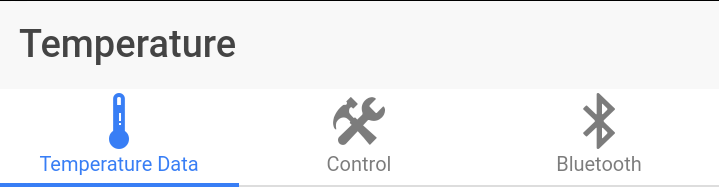
\includegraphics[scale=0.4]{pasekGora.png}
	\caption{Menu zakładek}
\end{figure}
Do przygotowania menu zakładek wykorzystano znaczniki \textit{<ion-tabs>}. Wyświetlenie treści odbywa się przez przełączanie widoku między stanami opisanymi na początku tego rozdziału.
\lstset{language=HTML}.
\begin{lstlisting}
<ion-tabs class="tabs-icon-top tabs-color-active-positive">
  <ion-tab title="Temperature Data" icon-off="ion-thermometer" icon-on="ion-thermometer" href="#/tab/temperature">
    <ion-nav-view name="tab-temperature"></ion-nav-view>
  </ion-tab>
  <ion-tab title="Control" icon-off="ion-settings" icon-on="ion-settings" href="#/tab/light">
    <ion-nav-view name="tab-light"></ion-nav-view>
  </ion-tab>
  <ion-tab title="Bluetooth" icon-off="ion-bluetooth" icon-on="ion-bluetooth" href="#/tab/bluetooth">
    <ion-nav-view name="tab-bluetooth"></ion-nav-view>
  </ion-tab>
</ion-tabs>
\end{lstlisting}
Do każdego z trzech przycisków przypisano nazwę i obrazek symbolizujący treść strony. Aktywna zakładka jest podświetlona w kolorze niebieskim.
\section{Strona pomiarowa}% jest ok
Strona pomiarowa służy wyłącznie do odczytu danych oraz ich wizualizacji. Struktura strony została zbudowana w sposób modułowy.
\begin{figure}[H]
	\centering
	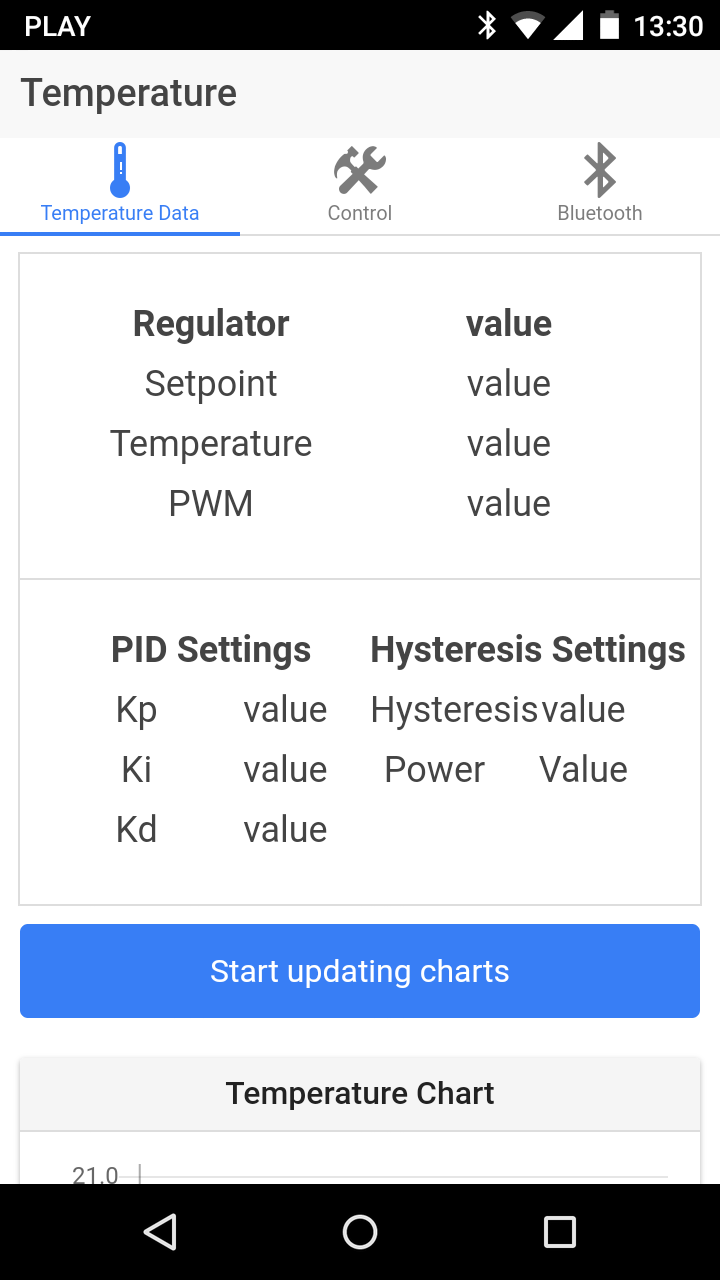
\includegraphics[scale=0.175]{apka1.png}
	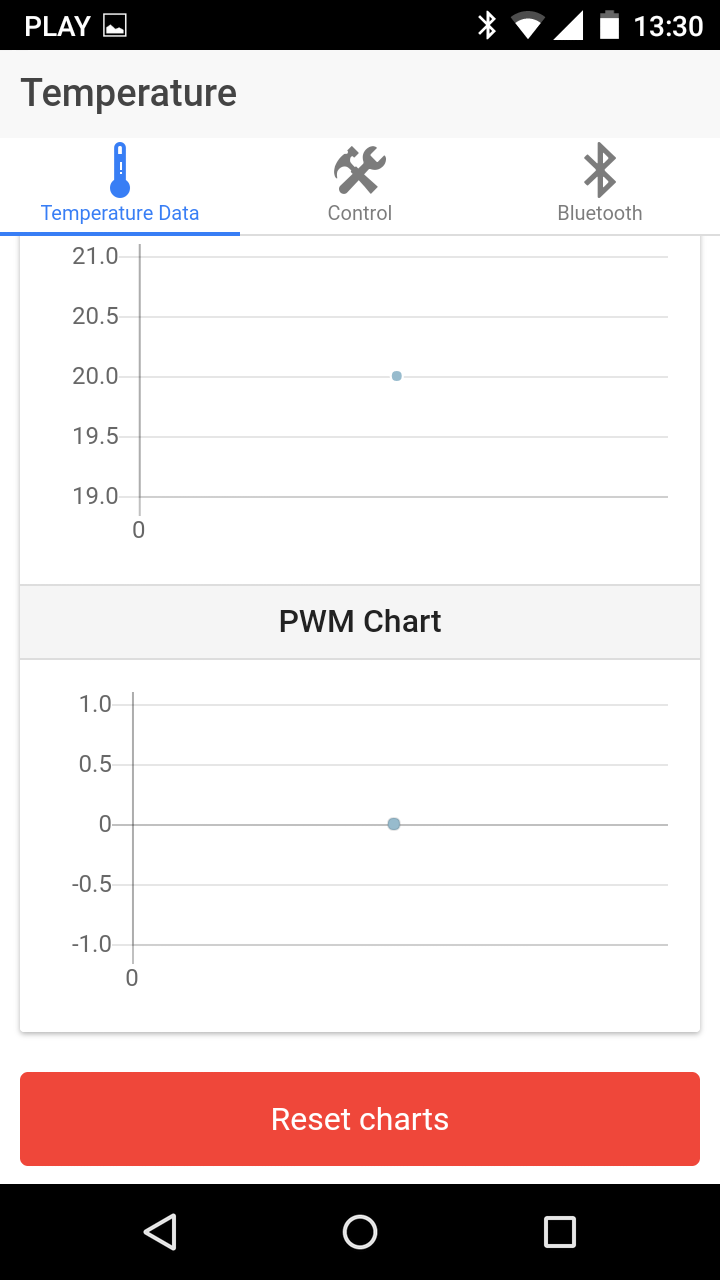
\includegraphics[scale=0.175]{apka2.png}
	\caption{Zakładka \textit{Temperature Data}}
\end{figure}
Podczas pracy układu regulacji bardzo ważna jest możliwość szybkiego odczytania aktualnych pomiarów i nastaw regulatorów. Dlatego, na początku zakładki umieszczono dwie tabele. Pierwsza z nich zawiera informacje ogólne, a druga specyficzne dla danego regulatora. Zamiast standardowych znaczników HTML, do utworzenia tabeli użyto znaczników \textit{div} oraz stylów mających odwzorować tabelę. Szerokość poszczególnych kolumn jest dopasowywana do wielkości wyświetlacza. Wyświetlane wartości zostały powiązane z kontrolerem \textit{TempCtrl} dzięki usłudze \textit{scope}. Takie rozwiązanie pozwala na uaktualnianie ich, po odebraniu nowych danych. 

Proces regulacji temperatury może zająć od kilku do kilkunastu minut. Dane wyświetlane w tabeli nie przekażą użytkownikowi informacji o tym, jak przebiegał proces w ostatnim okresie czasu. Za najciekawsze rozwiązanie uznano wizualizację danych na dwóch wykresach. Pierwszym przedstawiającym temperaturę aktualną i zadaną, a drugi sygnał sterujący PWM.
\begin{lstlisting} 
  <div class="card">
    <div class="item item-divider">
      Temperature Chart
    </div>
    <div class="item item-text-wrap">
      <canvas id="line1" class="chart chart-line" chart-data="data1" chart-labels="labels1" chart-legend="true" chart-series="series1" chart-options="options1"></canvas>
    </div>
    <div class="item item-divider">
      PWM Chart
    </div>
    <div class="item item-text-wrap">
      <canvas id="line2" class="chart chart-line" chart-data="data2" chart-labels="labels2" chart-legend="true" chart-series="series2" chart-options="options2"></canvas>
    </div>
  </div>
  <button class='button button-block button-assertive' ng-click="resetChart()">
    Reset charts
  </button>
\end{lstlisting}
Wykresy są dynamicznie aktualizowane, co trzecią pobraną próbkę danych. Ilość danych na wykresach ograniczono do 150 próbek, pozwalających na czytelne przedstawienie przebiegu procesu w ostatnich minutach. Po przekroczeniu zadanej ilości punktów, najstarsza informacja zostaje usunięta z wykresu. Do wyświetlenia grafów użyto znaczników \textit{<canvas>}, pozwalających na rysowanie wykresów przez JavaScript. Opcje dotyczące wykresów zostały sprecyzowane w kontrolerze strony.Ostatnim elementem strony jest przycisk \textit{Reset charts}, pozwalający na usunięcie wszystkich danych wyświetlonych na wykresach.

\subsection{Kontroler TempCtrl}%jest ok
TempCtrl to kontroler odpowiadający za możliwość ingerencji w interfejs użytkownika na stronie \textit{Temperature Data}. Odpowiedzialny jest za aktualizację wyświetlanych danych. W kontrolerze wykorzystano usługi:
\begin{itemize}
\item \textit{\$scope}- odpowiedzialny za połączenie kontrolera z widokiem użytkownika,
\item \textit{\$interval}- pozwala na wykorzystanie timerów,
\item \textit{receivedData}- serwis wykorzystywany do pobierania informacji,
\item \textit{bluetoothInformation}- serwis zawierający informację o aktualnym połączeniu Bluetooth.
\end{itemize}
Podobnie jak program mikrokontrolera Arduino, blok kontrolera posiada kod, który zostaje wykonany tylko raz, zaraz po pierwszym otwarciu zakładki. Wszystkim wyświetlanym parametrom, nadano wartość początkową \textit{value}. Sytuację przed pobraniem pierwszych próbek danych można zaobserwować na rysunku 6.1.
\lstset{language=Java}
\begin{lstlisting} 
	$scope.labels1 = [timeX];
	$scope.series1 = [['Actual Temperature'],['Setpoint']];
	$scope.data1=[[22],[22]];
	$scope.colors = ['#ff6384','#ff6384'];

	$scope.labels2 = [timeX];
	$scope.series2 = ['PWM'];
	$scope.data2=[0];
	$scope.color2 = ['#ff6384'];
\end{lstlisting}
W celu zainicjowania wykresów, wprowadzono na nie pierwszy punkt pomiarowy z aktualnym czasem i wartością mieszczącą się w zakresie pracy. Dodatkowo określono nazwy i kolory serii danych. Modyfikacja wyglądu wykresów nastąpiła poprzez przypisanie opcji do zmiennych \textit{\$scope.options} każdego wykresu. Oś Y umieszczono po lewej stronie. Ilość etykiet na osi X ograniczono do 4. W celu poprawienia płynności działania wykresów, wyłączono funkcję animacji rysowania nowego punktu.
\begin{lstlisting} 
	var interval1=$interval(receiveData, 1000);
\end{lstlisting}
Uruchomiony został również jedyny interwał wykonywany w tym kontrolerze. Funkcja \textit{receiveData} wykorzystuje usługę receivedData do pobrania nowych pomiarów z bufora modułu Bluetooth. Działanie cyklicznie wykonywanej funkcji zaczyna się od wykonania metody \textit{receivedData.getData()}, która pobiera i przetwarza dane. Następnie warunek \textit{if} sprawdza czy, odebrana paczka danych była kompletna. Jeśli tak, to wyświetlane wartości zostają zaktualizowane przy użyciu metod \textit{getKp, getTemperature} itd. Informacja o aktualnie pracującym regulatorze zostaje odebrana w postaci liczby, która w zależności od wartości zostaje zamieniona na tekst \textit{Hysteresis} lub \textit{PID}. Na końcu program sprawdza czy, było to już trzecie wywołanie funkcji aktualizacji. Jeśli tak, to zmienna licząca jest zerowana, a następnie proces przechodzi do wykonania funkcji \textit{updateCharts}. W przypadku otrzymania niepoprawnych danych, proces aktualizacji zostaje pominięty.

Na początku działania funkcji \textit{updateCharts()}, aktualizowana jest zmienna \textit{timeX} przechowująca aktualny czas. Przed dodaniem nowego punktu, sprawdzana jest ilość danych na wykresie. Jeśli jest ona równa lub większa 150, to należy usunąć najstarszą narysowaną próbkę z obu wykresów. Metoda \textit{slice} wycina tablicę z pominięciem jej pierwszej komórki i zapisuje ją zamiast starej zmiennej. Działanie zostaje powtórzone dla każdej serii danych obu wykresów. Następnie do tablicy dopisane zostają najświeższe pomiary używając metody \textit{push}.

Do przycisku \textit{Reset charts} za pomocą zdarzenia \textit{ng-click} przypisano funkcję \textit{resetChart} nadpisującą zestawy danych każdego z wykresów, ostatnio pobranymi wartościami.

\section{Zakładka konfiguracyjna}%jest ok
Zakładka konfiguracyjna została utworzona w celu możliwości wygodnego zmieniania temperatury zadanej, wyboru typu regulatora i jego nastaw. Wybrane ustawienia zostają przesłane do układu mikroprocesorowego, po użyciu przycisku \textit{Confirm new setting}.

Strukturę strony ponownie oparto o style dostępne w frameworku. Panel wyboru typu regulatora został utworzony za pomocą klasy \textit{item-select} i znaczników \textit{<select>}, do których przy pomocy polecenia \textit{ng-model} przypisano zmienną widoczną dla kontrolera tej karty.
\begin{figure}[H]
	\centering
	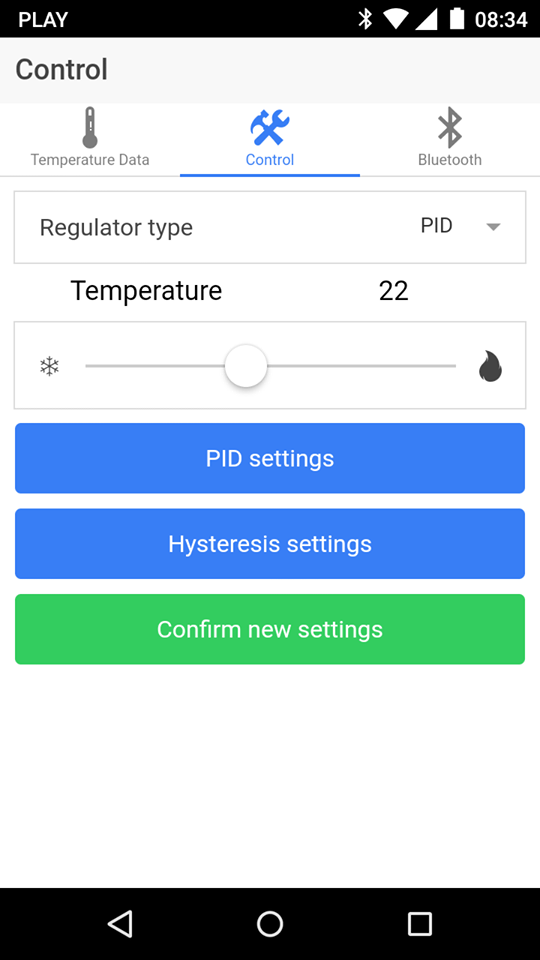
\includegraphics[scale=0.25]{apka3.png}
	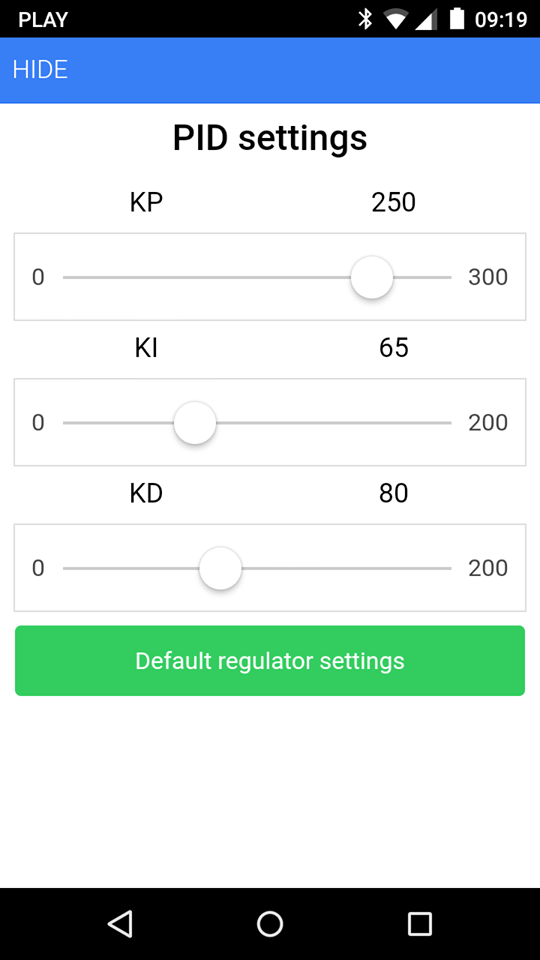
\includegraphics[scale=0.25]{apka4.png}
	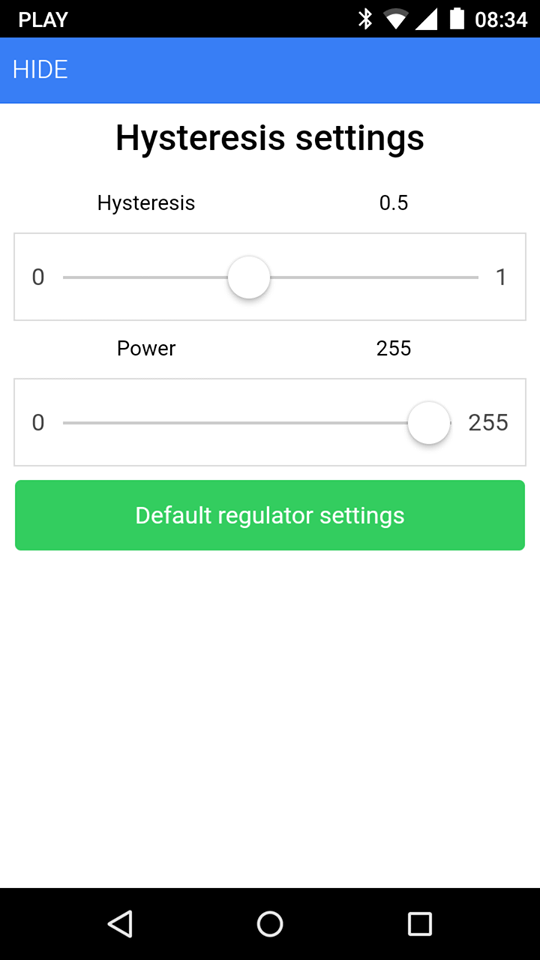
\includegraphics[scale=0.25]{apka5.png}
	\caption{Zakładka \textit{Control}}
\end{figure}


Za pomocą znacznika \textit{<input>} typu \textit{range} utworzono suwak regulacji temperatury zadanej. Po lewej stronie suwaka umieszczono ikonę płatka śniegu oznaczającego niską temperaturę, a z prawej strony płomień oznaczający wysoką temperaturę.

Kolejnymi elementami interfejsu są 2 przyciski. Każdy z nich otwiera nowy \textit{modal}. \textit{Modal}, to nowe okno widoku, pojawiające się nad głównym interfejsem użytkownika. Pierwszy z przycisków tworzy \textit{modal}, w którym ponownie umieszczono suwaki konfiguracji wzmocnień \textit{kp}, \textit{ki} i \textit{kd} regulatora PID. Pod suwakami umieszczono przycisk \textit{Default regulator settings}, pozwalający na przywrócenie standardowych nastaw regulatora. Modal odpowiadający drugiemu przyciskowi, został zaprojektowany w podobny sposób, ale zawiera on parametry regulatora histerezowego. Trzeci obiekt to przycisk potwierdzenia ustawień, który został wyróżniony zielonym kolorem. Zaakceptowanie ustawień jest potwierdzane komunikatem.

Struktura użytych \textit{modali} została zapisana w pliku HTML tej zakładki. Każdemu z nich został przydzielony indywidualny numer \textit{id}.

\subsection{Kontroler ControlCtrl} %jest ok
W celu poprawnego działania kontrolera użyto w nim usługi \textit{\$scope} oraz \textit{\$ionicModal}. Na początku bloku kontrolera utworzono zmienne powiązane z widokiem aplikacji, odpowiedzialne za wartości konfigurowane za pomocą suwaków i panelu wyboru. Ze względu na sposób działania wejścia w postaci suwaka, dane musiały zostać zapisane w  postaci obiektowej.
\begin{lstlisting} 
	var regulator=1;
	$scope.data={'regulatorType':'PID'};
	$scope.data1={'newSetpoint':'22'};
	$scope.data2={'kp':'15'};
	$scope.data3={'ki':'5'};
	$scope.data4={'kd':'2'};
	$scope.data5={'hyst':'0.25'}
	$scope.data6={'power':'255'}
\end{lstlisting}
Do zmiennych \textit{oModal1} i \textit{oModal2} przypisano modale utworzone w pliku HTML tej strony. Do zidentyfikowania ich został wykorzystany parametr \textit{id}.

Do przycisków odpowiedzialnych za wyświetlanie nowych okien, przypisano funkcję \textit{openModal()}, przyjmującą jako argument numer okna do otwarcia. Dla argumentu równego 1 zostaje otwarty widok konfiguracji regulatora PID, a dla 2 okno regulatora histerezowego. Wydarzeniem wykonywanym po naciśnięciu przycisku \textit{Hide} znajdującego się w lewym, górnym narożniku jest funkcja \textit{closeModal()}, przyjmująca te same argumentu co w poprzednim przypadku. Okno zostaje ukryte dzięki metodzie \textit{hide()}. Podczas otwierania użyto \textit{show()}.

Szczególną rolę w tym kontrolerze pełni funkcja \textit{sendSetpoint()}, odpowiedzialna za przesłanie ramki przedstawionej na rysunku 5.2. W celu ograniczenia ilości przesyłanych znaków, nazwa regulatora zostaje zastąpiona przez cyfrę.
\begin{lstlisting}
bluetoothSerial.write("t"+$scope.data1.newSetpoint+"p"+$scope.data2.kp+"i"+$scope.data3.ki+"d"+$scope.data4.kd+"r"+regulator+"h"+$scope.data5.hyst+"m"+$scope.data6.power+"/n")
\end{lstlisting}
Ramka zostaje wysłana za pomocą metody \textit{bluetoothSerial.write}, w przedstawiony powyżej sposób.. W przypadku pozytywnie zakończonego procesu wysyłania danych, zostaje wyświetlony komunikat, informujący o przesłaniu danych. W przeciwnej sytuacji wyświetlone okno informacyjne zawiera komunikat o niepowodzeniu przesyłania danych.

\section{Bluetooth}
Ostatnia utworzona zakładka służy do konfiguracji modułu Bluetooth urządzenia mobilnego. Kontroler utworzony do obsługi wydarzeń na stronie, nazywa się \textit{BlueCtrl}. Interfejs składa się na przycisk wyszukiwania urządzeń oraz dwie sekcje:
\begin{itemize}
\item urządzenia sparowane z telefonem,
\item nowe wyszukane urządzenia.
\end{itemize}
\begin{figure}[H]
	\centering
	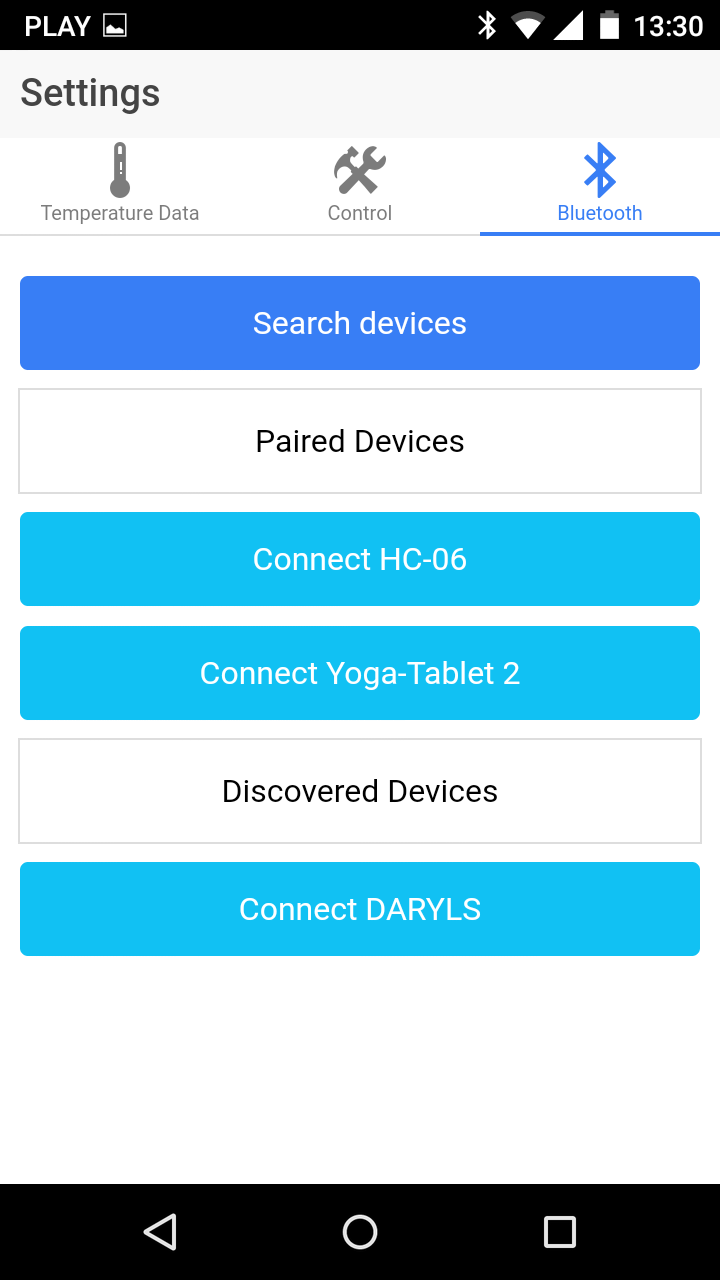
\includegraphics[scale=0.175]{apka6.png}
	\caption{Zakładka \textit{Bluetooth}}
\end{figure}
Program znajdzie wszystkie dostępne w okolicy urządzenia, ale nawiązanie komunikacji możliwe jest jedynie z modułem slave, podłączonym do Arduino. Do przycisku przypisano wydarzenie \textit{ng-click}, odwołujące się do funkcji \textit{findDevices()}, która została szerzej opisana w rozdziale poświęconym kontrolerowi \textit{BlueCtrl}. 
\lstset{language=HTML}
\begin{lstlisting}
<button ng-repeat="device in pairedDevices" ng-click="connectMac({{device}})" class='{{typeConnect}}'>
	{{textConnect}} {{device.name}}
</button>
\end{lstlisting}
W pliku HTML utworzono dwa przyciski, które początkowo są niewidoczne, dlatego że przypisane im obiekty nie zawierają jeszcze żadnych elementów. Po użyciu przycisku wyszukiwania, obiekty zostają wypełnione znalezionymi urządzeniami. Za pomocą dyrektywy \textit{ng-repeat} utworzony szkielet przycisku zostaje powielony dla każdego obiektu w obiekcie. Następnie każdy przycisk zostaje zidentyfikowany przez nazwę i adres urządzenia.

Po wciśnięciu wygenerowanego przycisku wywołana zostaje funkcja \textit{connectMac()}, przyjmująca jako argument obiekt, przypisany do przycisku.


\subsection{Kontroler BluetoothCtrl}


W celu dodatkowego zabezpieczenia poprawnej funkcjonalności aplikacji poza standardowymi usługami \textit{\$scope} i \textit{\$timeout}, użyto jeszcze serwisu \textit{\$ionicLoading} i \textit{bluetoothInformation}. Po uruchomieniu zakładki po raz pierwszy, powstają zmienne przechowujące bazowy wygląd przycisku połączenia z urządzeniem. Następnie po opóźnieniu równym 0.5 sekundy zostaje wykonana metoda \textit{bluetoothInformation.isBluetoothON()}, sprawdzająca czy moduł jest uruchomiony. Funkcja została opóźniona dlatego, że  wtyczka \textit{bluetoothSerial} jest dostępna dla aplikacji z minimalnym opóźnieniem. W przeciwnym wypadku metoda usługi zostały nierozpoznana.

Funkcja odpowiedzialna za wyszukiwanie nowych urządzeń została zabezpieczona przez warunek \textit{if}, ponownie sprawdzający czy moduł jest uruchomiony. Jeśli zostanie zwrócona wartość pozytywna, to ekran zostaje zablokowany przez proces wczytywania uruchomiony przez usługę \textit{\%ionicLoading}.  Zastosowano takie rozwiązanie w celu uniknięcia sytuacji, w której użytkownik wielokrotnie używa przycisku, zamiast zaczekać, aż funkcja zakończy pracę.

\begin{lstlisting}
bluetoothSerial.list(function (data) {
	console.log("List: "+data);
	$scope.$apply(function () {
		$scope.pairedDevices=data})},function () {
		console.log("No devices found");
	});
\end{lstlisting}
Lista wygenerowana przez metodę \textit{bluetoothSerial.list()} zostaje przekazana w formie argumentu \textit{data} do kolejnej funkcji. Otrzymane dane zapisane są w postaci obiektowej.Metoda wyszukująca dostępne urządzenia działa dokładnie w ten sam sposób. Po wykonaniu drugiej komendy, niezależnie od poprawności jej wykonania, ekran zostaje odblokowany. Dla zapewnienia poprawności działania aplikacji, a dokładniej wyświetlenia przycisków, aktualizacja uzyskanych danych do DOM, zostaje wymuszona przez polecenie \textit{\$scope.\$apply}.

Kolejną ważną funkcją powiązaną z elementami strony HTML jest polecenie \textit{connectMac(obiekt)}, które jako argument przyjmuje obiekt opisujący dane urządzenie. Po wywołaniu wydarzenia, ekran zostaje ponownie zablokowany. Następnie wykonywana jest usługa sprawdzająca status połączenia. W kolejnym kroku warunek \textit{if} sprawdza zwróconą wartość, opisującą status połączenia. Cześć usługi wykonującej funkcję sprawdzenia i część zwracająca wynik rozdzielono na dwie osobne metody ze względu na pojawiające się opóźnienie w przypisaniu danych. W zależności od spełnienia lub nie warunku, zostaje wywołana część bloku odpowiedzialna za rozłączenie z urządzeniem lub połączenie z nim. Każda uzyskana odpowiedź powoduje wyświetlenie się alertu informującego o wyniku przeprowadzonej operacji. W przypadku pozytywnego skutku rozłączenie lub niepowodzenia w połączeniu, zostaje wywołana funkcja \textit{checkConnection1()}, zmieniająca wygląd przycisków do postaci początkowej. Dla niepowodzenia w rozłączeniu i prawidłowego nawiązania połączenia zostaje wykonana funkcja \textit{checkConnection()}, która za pomocą usługi \textit{bluetoothInformation} sprawdza status połączenia i dopasowuje do niego wygląd przycisków. Następnie ekran aplikacji zostaje odblokowany.



%%%%%%%%%%%%%%%%%%%%%%%%	Testy działania
\chapter{Przeprowadzone testy}
Pierwszym przeprowadzonym testem było sprawdzenie wydajności układu podczas procesu chłodzenia obiektu.
\begin{figure}[H]
	\centering
	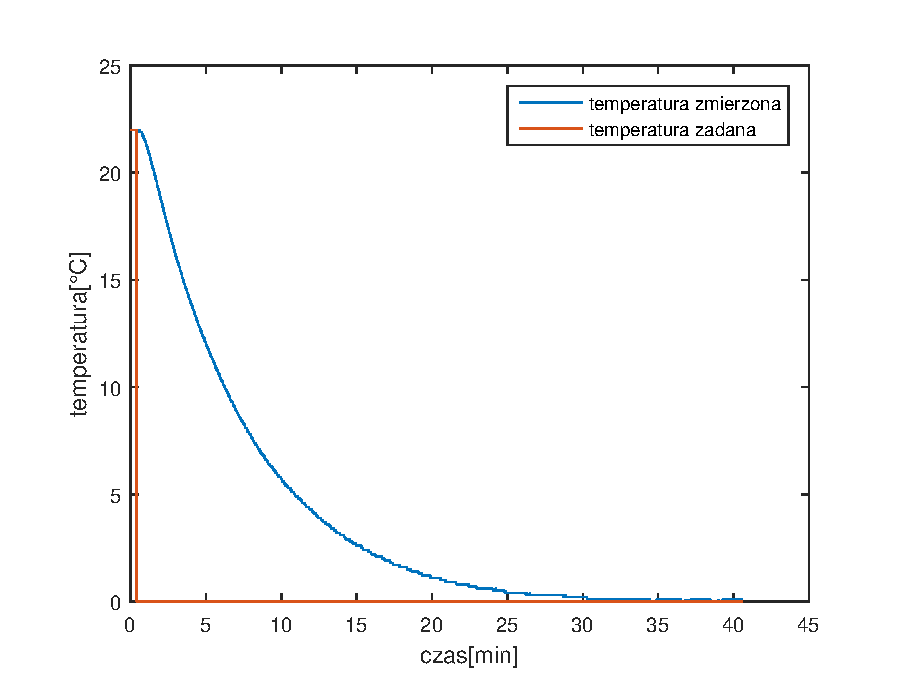
\includegraphics[scale=0.75]{test_chlodzenia.eps}
	\caption{Test wydajności układu regulacji temperatury}
	\label{fig:chlodzenie}
\end{figure}
Podczas całego procesu ogniwo pracowało z pełną mocą. Proces rozpoczął się od ustabilizowania temperatury na 22 stopniach Celsjusza. Następnie, na sterownik ogniwa zadano sygnał PWM o maksymalnej częstotliwości. Na rysunku 7.1 można zaobserwować, że obiekt został bardzo szybko schłodzony do temperatury poniżej 10 stopni. Granicą wydajności okazała się temperatura zbliżona do zera, na której odczyt ustabilizował się po 35 minutach. Osiągnięta wartość okazała się znacznie niższa niż przewidywano.

Ze względu na duże temperatury osiągane przez ogniwo (do ponad $100^{\circ} C$) podczas ogrzewania zdecydowano, że test maksymalnej osiągniętej temperatury w obiekcie nie zostanie przeprowadzony.
\section{Regulator histerezowy}
W pierwszej kolejności przetestowano najbardziej podstawowy regulator- histerezowy. Otrzymane wyniki są zbliżone do temperatury zadanej. Regulator histerezowy charakteryzuje się dużą stabilnością przebiegu, którą można zaobserwować na rysunku ~\ref{fig:hist18} i ~\ref{fig:hist26}.
\begin{figure}[H]
	\centering
	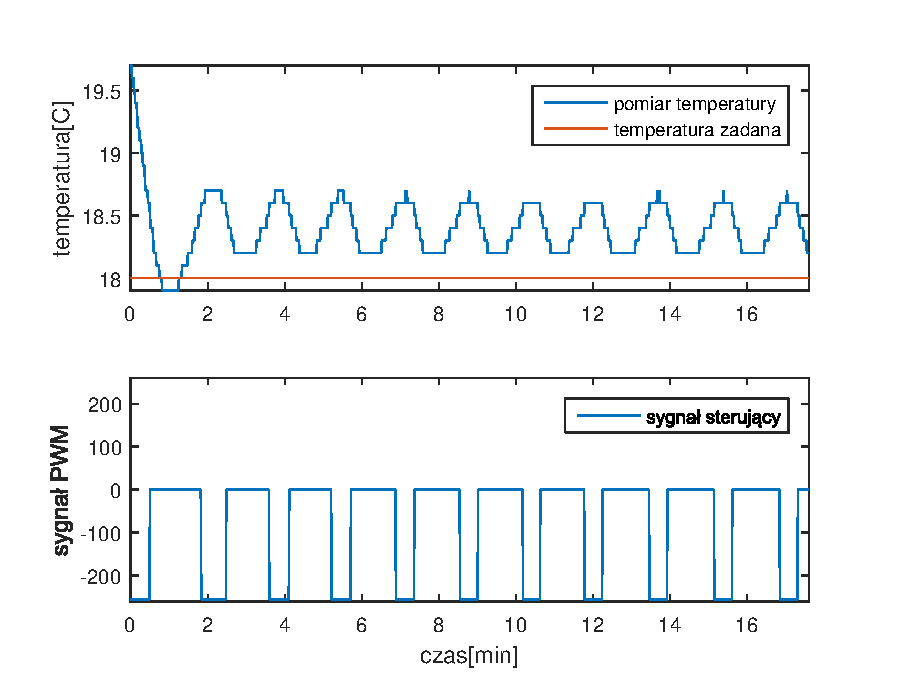
\includegraphics[scale=0.8]{hist18.eps}
	\caption{Regulator histerezowy. Histereza 0.5 stopnia.}
	\label{fig:hist18}
\end{figure}

\begin{figure}[H]
	\centering
	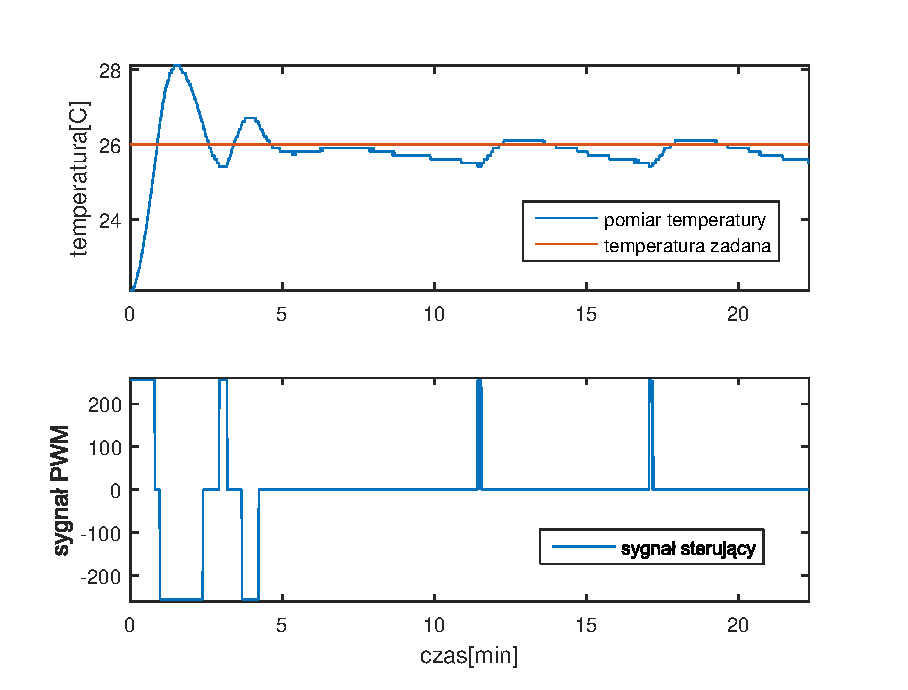
\includegraphics[scale=0.8]{hist26.eps}
	\caption{Regulator histerezowy. Histereza 0.5 stopnia.}
	\label{fig:hist26}
\end{figure}
\newpage
\section{Regulator PID}
Test regulatora PID został podzielony na etapy, w których przetestowano wpływ nastaw regulatora na działanie każdego z członów. Podczas testów członu całkującego i różniczkującego wykorzystano również człon proporcjonalny.

\subsection{P}
\begin{figure}[H]
	\centering
	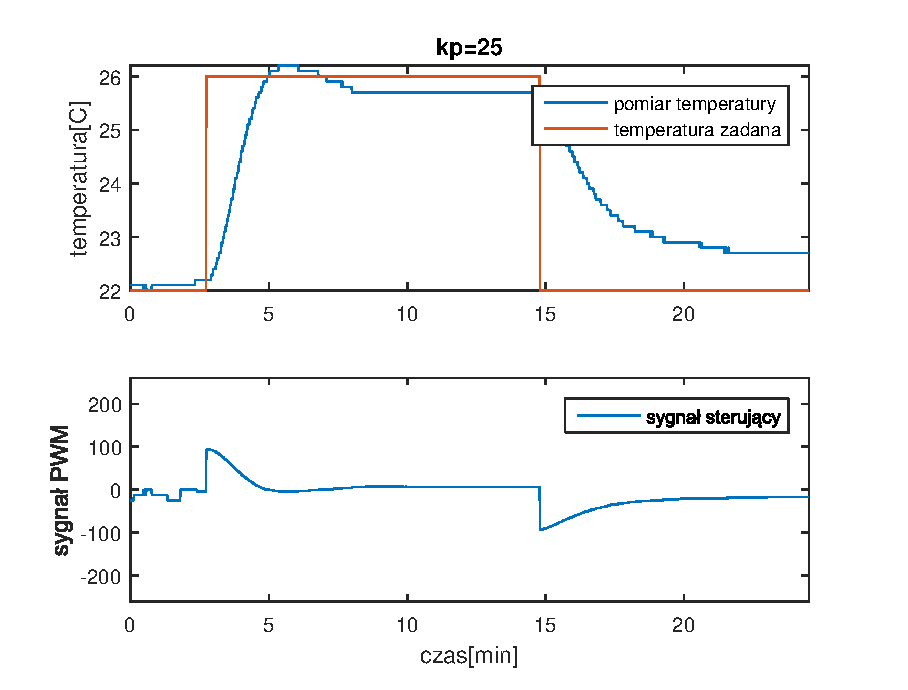
\includegraphics[scale=0.9]{26kp25.eps}
	\caption{Regulator P, kp=25}
	\label{fig:kp25}
\end{figure}
Na rysunku ~\ref{fig:kp25} można zaobserwować, że dla niskiej wartości wzmocnienia członu proporcjonalnego,temperatura szybko stabilizuje się, ale na poziomie niższym od zadanego. Przy wartości kp=25, regulator nie jest w stanie osiągnąć zadanej temperatury podczas procesu chłodzenia.
\newpage
\begin{figure}[H]
	\centering
	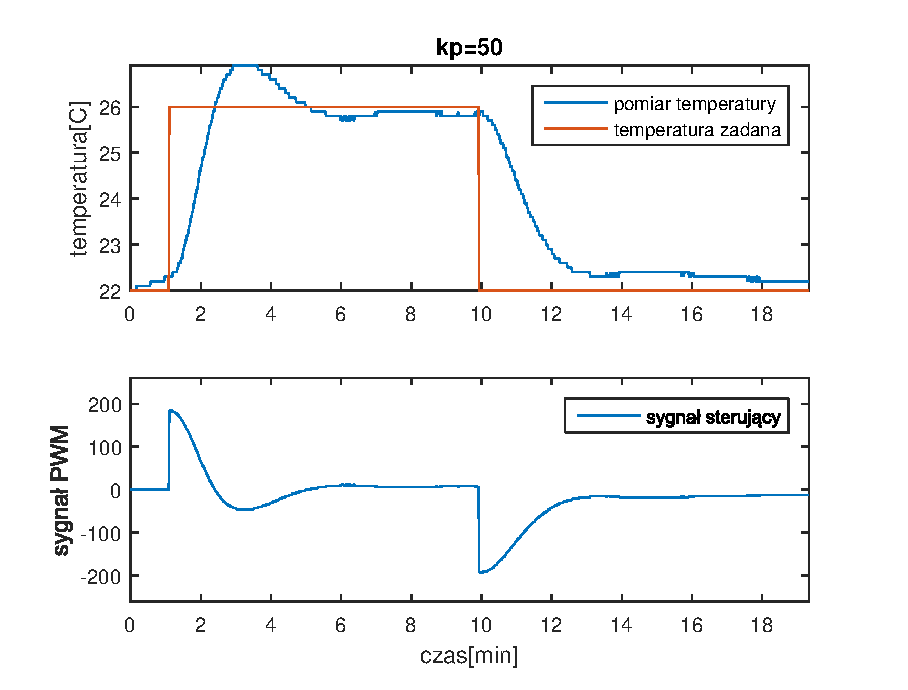
\includegraphics[scale=0.9]{26kp50.eps}
	\caption{Regulator P, kp=50}
	\label{fig:kp50}
\end{figure}
\begin{figure}[H]
	\centering
	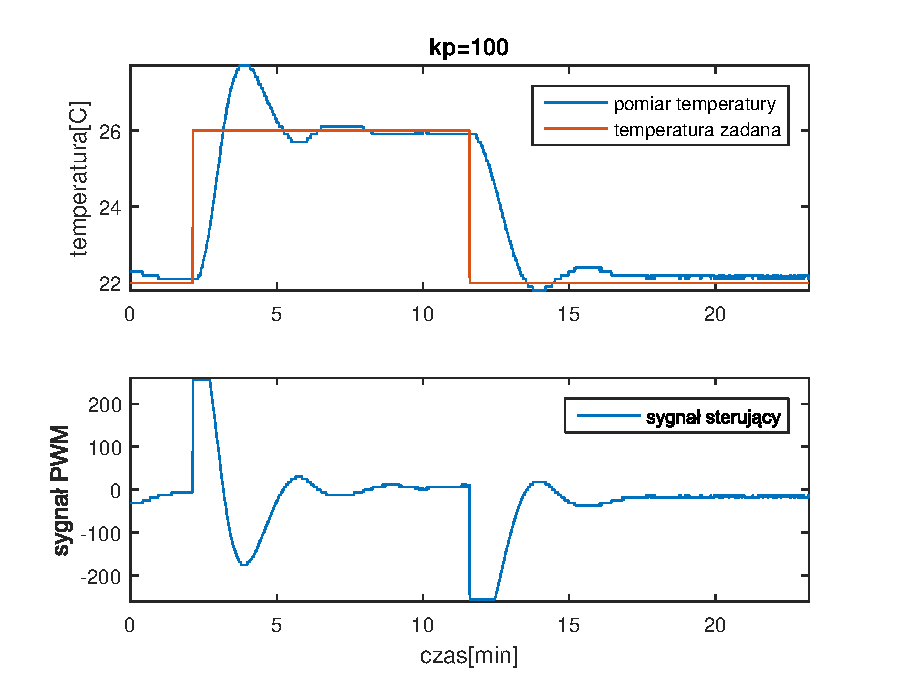
\includegraphics[scale=0.9]{26kp100.eps}
	\caption{Regulator P, kp=100}
\end{figure}
\begin{figure}[H]
	\centering
	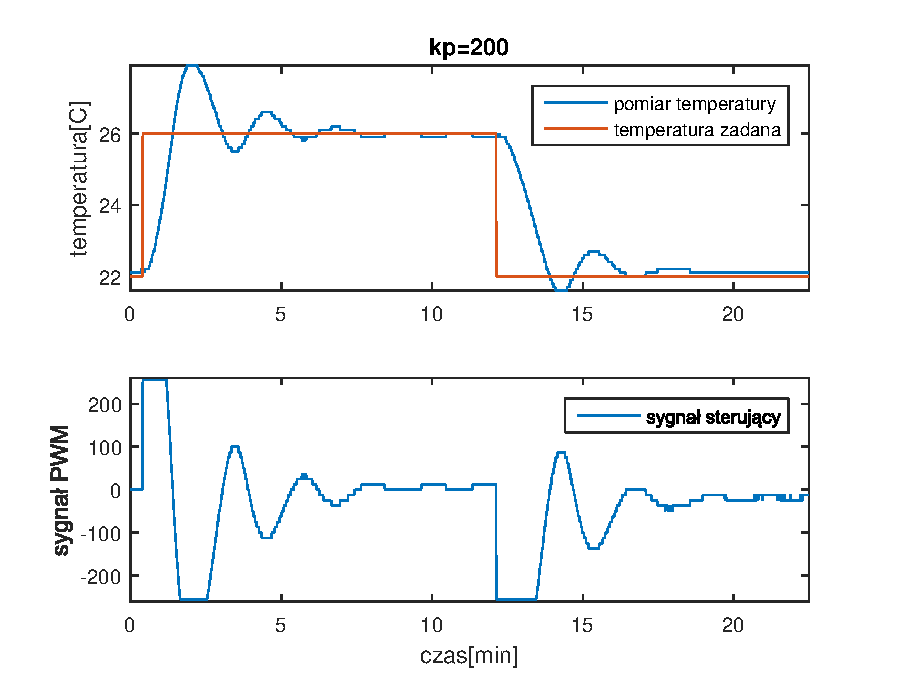
\includegraphics[scale=0.9]{26kp200.eps}
	\caption{Regulator P, kp=200}
	\label{fig:kp200}
\end{figure}
Po zwiększeniu wzmocnienia do 50, na rysunku ~\ref{fig:kp50} można zaobserwować nieznaczną poprawę czasu narastania, ale pojawiły się niedogodności w postaci przeregulowania na poziomie $1^{\circ} C$. Tym razem temperatura  ustaliła się bliżej wartości zadanej. Proces chłodzenia również przebiegł znacznie sprawniej.

Kolejne dwukrotne zwiększenia nastawy regulatora spowodowało znaczne skrócenie czasu narastania, ale wydłużyło czas regulacji. Przeregulowania przekroczyły wartość $2^{\circ} C$. Na charakterystyce pojawiły się powoli tłumione oscylacje temperatury.
\newpage

\subsection{PI}

\begin{figure}[H]
	\centering
	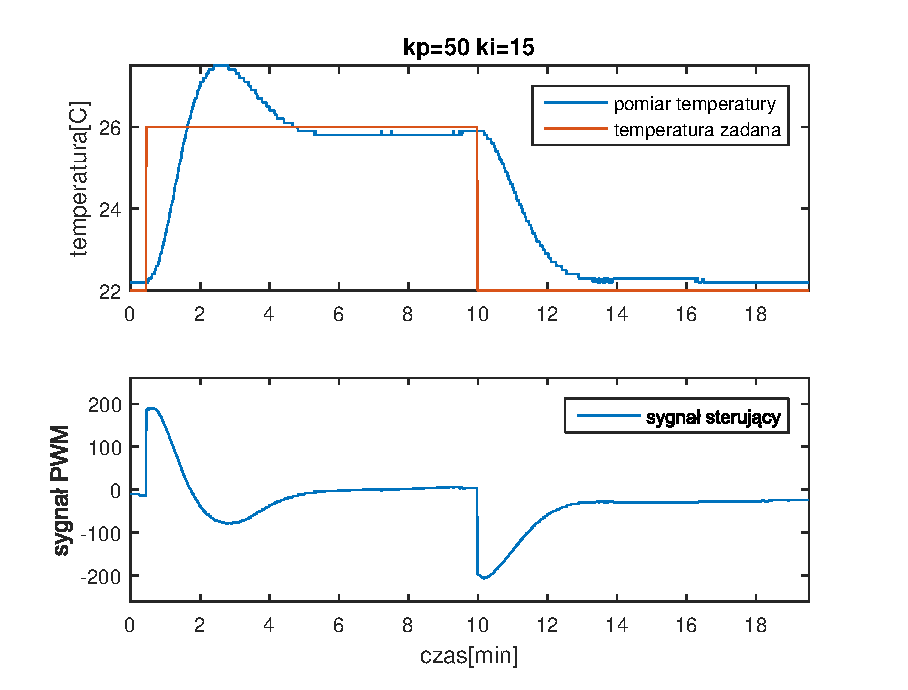
\includegraphics[scale=0.9]{26kp50ki15.eps}
	\caption{Regulator PI, kp=50 ki=15}
	\label{fig:ki15}
\end{figure}
\begin{figure}[H]
	\centering
	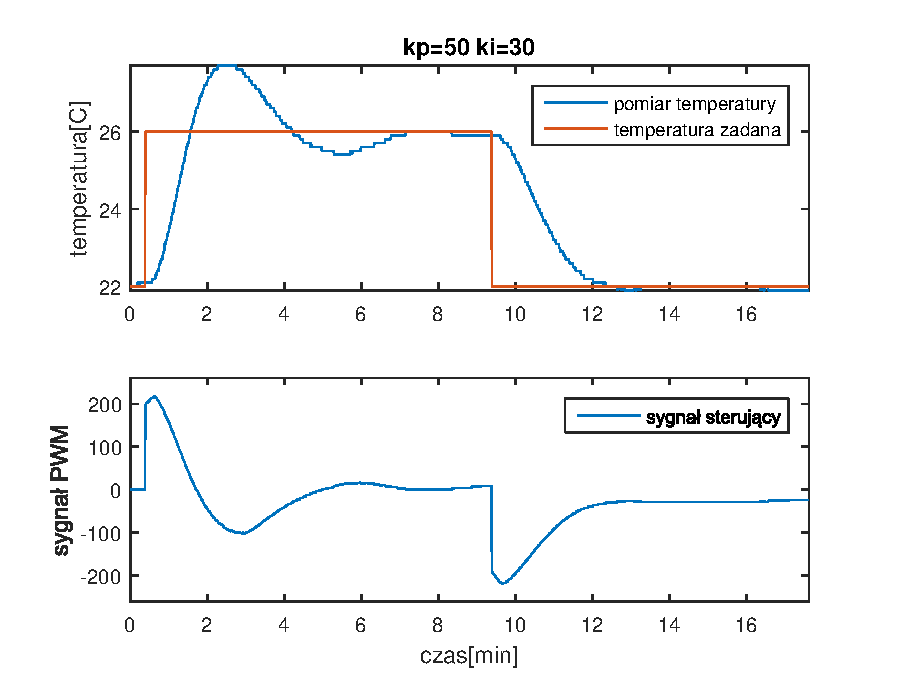
\includegraphics[scale=0.9]{26kp50ki30.eps}
	\caption{Regulator PI, kp=50 ki=30}
	\label{fig:ki30}
\end{figure}

Wprowadzenie członu całkującego o małej wartości (rysunek ~\ref{fig:ki15}), wyraźnie skróciło czas narastania. Dodatkowym skutkiem okazało się przybliżenie wartości otrzymanej do oczekiwanej, również podczas chłodzenia. Znacznym problemem wykorzystanych nastaw jest narastanie członu całkującego, który później powoduje powstanie znacznych przeregulowań.

Podczas kolejnego testu, zwiększono wzmocnienie całkujące do 30. Przeregulowanie nieznacznie wzrosło. Czas regulacji wydłużył się z powodu pojedynczej oscylacji, widocznej na rysunku ~\ref{fig:ki30}. Temperaturę można uznać za prawidłowo wyregulowaną. Po ustaleniu się, odstępstwa od wartości zadanej wynosiły jedynie 0.1 stopnia, co jest wartością bardzo zadowalającą dla pomiaru wykonywanego z dokładnością +/- 0.5 stopnia.

Kolejne zwiększenie nastawy \textit{ki} przedstawione na rysunku ~\ref{fig:ki60}, nie przyniosło pozytywnych efektów. Podczas ogrzewania zaobserwowano wielokrotne przeregulowania. Oscylacje pojawiły się również podczas ochładzania obiektu. Czas narastania skrócił się, a czas regulacji znacznie wydłużył.

\begin{figure}[H]
	\centering
	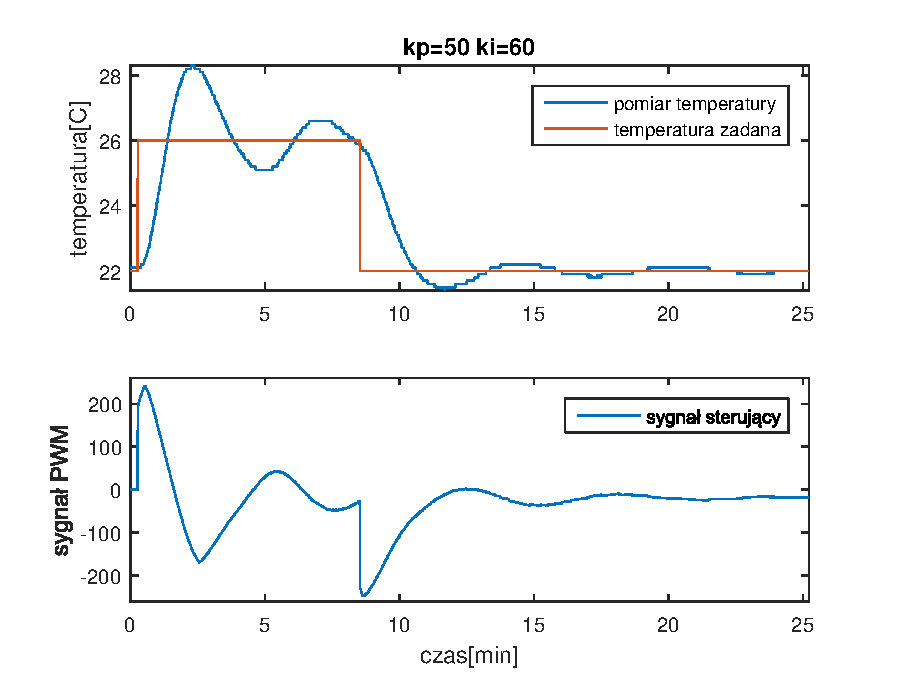
\includegraphics[scale=0.9]{26kp50ki60.eps}
	\caption{Regulator PI, kp=50 ki=60}
	\label{fig:ki60}
\end{figure}

Najkorzystniejszym rozwiązaniem okazała się pośrednia wartość wzmocnienia członu całkującego. Dla wartości zbyt małej, efekty włączenia członu I są praktycznie niewidoczne. Wprowadzenie dużego wzmocnienia zmniejsza ostateczny błąd regulacji, kosztem pojawienia się licznych oscylacji i znacznego wydłużenia procesu regulacji.
\newpage

\subsection{PD}
Pierwszy test członu różniczkującego przebiegł zgodnie z oczekiwaniami. Na rysunku ~\ref{fig:kp200} można zaobserwować, że wzmocnienie \textit{kp}=200 spowodowało pojawienie się dużego przeregulowania oraz oscylacji. W przykładzie z rysunku ~\ref{fig:kd20}, wartość wzmocnienia proporcjonalnego zwiększono o kolejne 50 jednostek. Po dodaniu członu D, przebieg temperatury został spłaszczony i ustalił się szybciej niż dla samego członu P.
\begin{figure}[H]
	\centering
	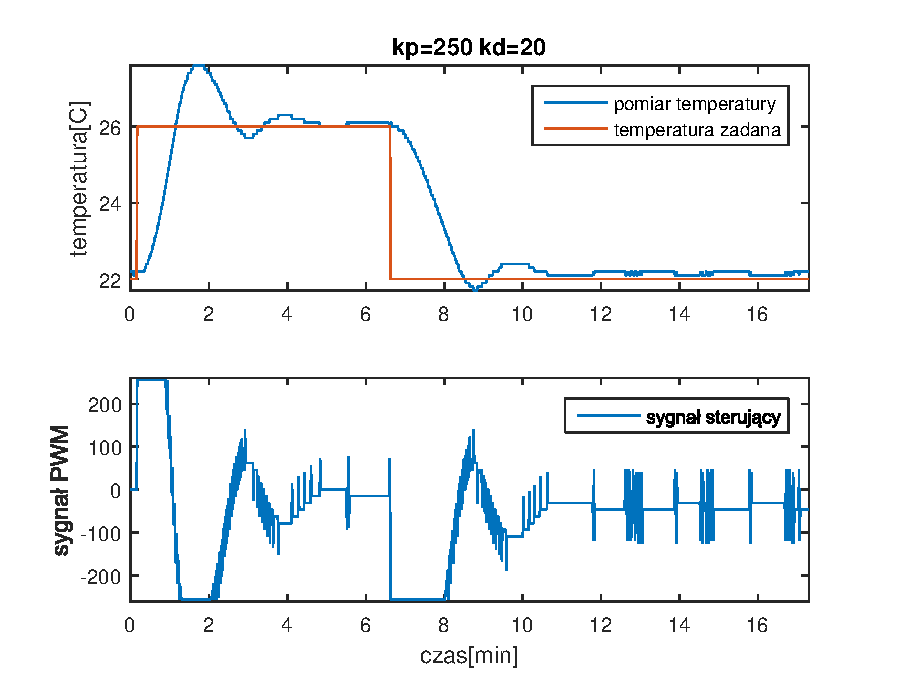
\includegraphics[scale=0.9]{26kp250kd20.eps}
	\caption{Regulator PD, kp=250 kd=20}
	\label{fig:kd20}
\end{figure}
Kolejne zwiększenia wartości nastawy \textit{kd}, spowodowały znaczne zmniejszenie wartości przeregulowania oraz prawie całkowicie zniwelowały występowanie oscylacji.

Po ustawieniu parametru na 80 jednostek, przeregulowanie zostało ograniczone z  2 stopni Celsjusza do około 0.5 stopnia. Niestety, przy tak dużym wzmocnieniu członu D, temperatura ustala się powyżej wartości zadanej.
\newpage
\begin{figure}[H]
	\centering
	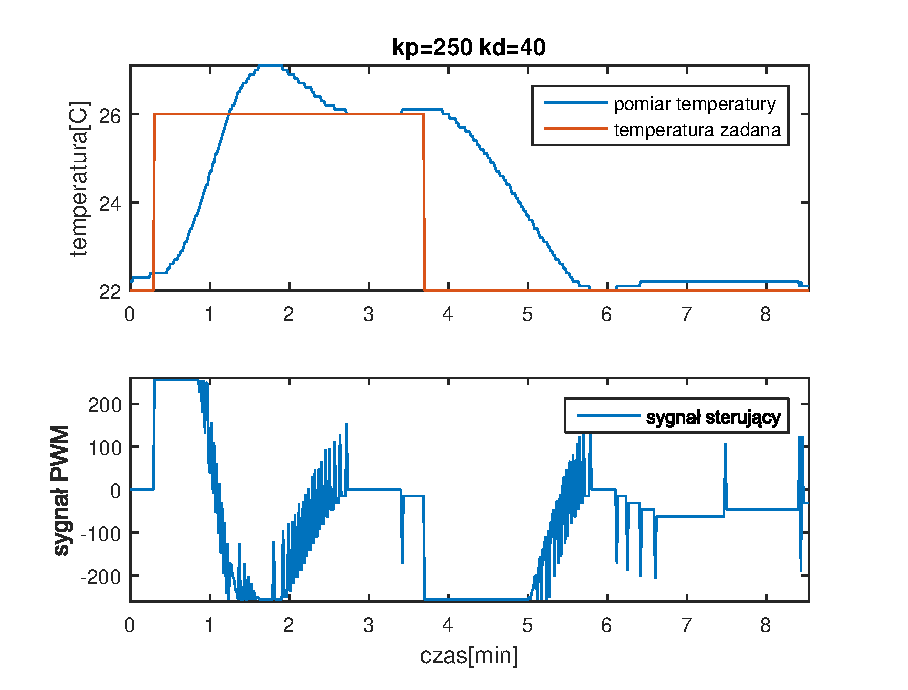
\includegraphics[scale=0.9]{26kp250kd40.eps}
	\caption{Regulator PD, kp=250 kd=40}
\end{figure}
\begin{figure}[H]
	\centering
	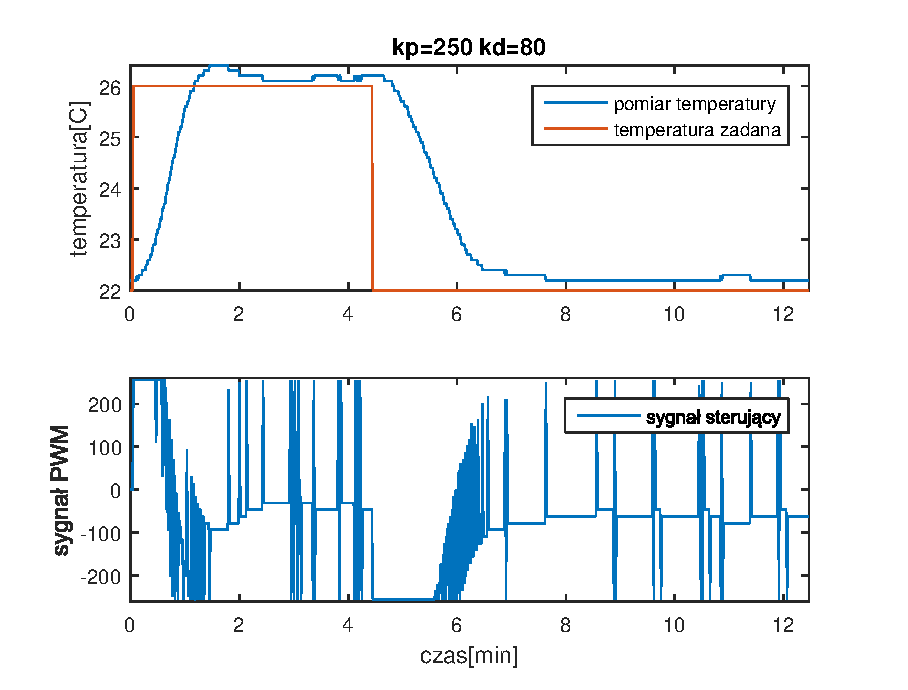
\includegraphics[scale=0.9]{26kp250kd80.eps}
	\caption{Regulator PD, kp=250 kd=80}
\end{figure}

\subsection{PID}
W celu zniwelowania niekorzystnych efektów używania członu I oraz D, należy wykorzystać regulator PID, który po dobraniu odpowiednich nastaw powinien pozwolić na ograniczenie przeregulowania oraz oscylacji, bez pogorszenia czasu narastania i regulacji temperatury.

Nastawy regulatora zostały dobrane ręcznie, po wykonaniu licznych prób i testów działania regulatora. Duża wartość parametru \textit{kp} i \textit{ki} pozwoliła na zmniejszenie czasu narastania poniżej 2 minut. Dzięki członowi \textit{D}, zmniejszono wartość przeregulowania. Odstępstwa temperatury zmierzonej od zadanej na poziomie +/-0.1 stopnia, uznano za bardzo dobry wynik.

Poniżej przedstawiono wybrane testy dla temperatur z przedziału od 18 do 30 stopni Celsjusza. Optymalne nastawy regulatora to: \textit{kp}=250, \textit{ki}=62, \textit{kd}=80.
%\begin{itemize}
%\item \textit{kp}=250,
%\item \textit{ki}=62,
%\item \textit{kd}=80.
%\end{itemize}
Podczas chłodzenia obiektu przeregulowanie nie występuje, a temperatura zostaje bardzo szybko zbliżona do zadanej. W kolejnych minutach temperatura stopniowo zbliża się do zadanej wartości. Pojawiające się na przebiegu sygnału sterującego \textit{szpilki}, są wynikiem działania części różniczkującej regulatora, w ten sposób hamowane jest narastanie temperatury podczas zbliżania się do wartości zadanej.
\begin{figure}[H]
	\centering
	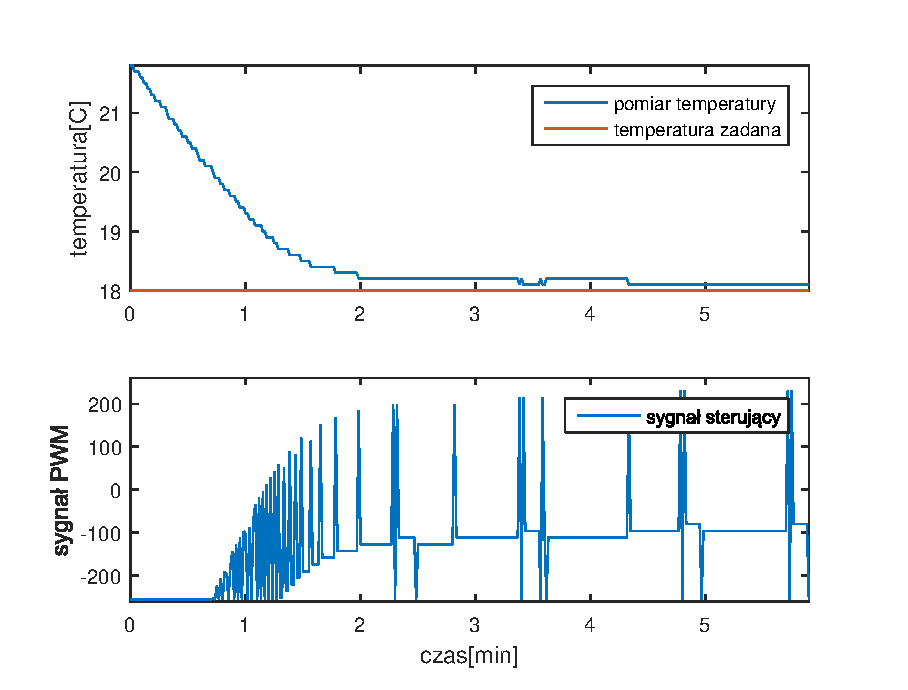
\includegraphics[scale=0.9]{pid18.eps}
	\caption{Regulacja dla $18^{\circ} C$}
	\label{fig:pid18}
\end{figure}
Na wykresie ~\ref{fig:pid30} można zaobserwować, że czas narastania i regulacji został bardzo mocno skrócony. Mimo dużej różnicy pomiędzy temperaturą początkową i zadaną, przeregulowanie nie przekroczyło 0.5 stopnia, a czas regulacji to jedynie około 3.5 minuty. 
\begin{figure}[H]
	\centering
	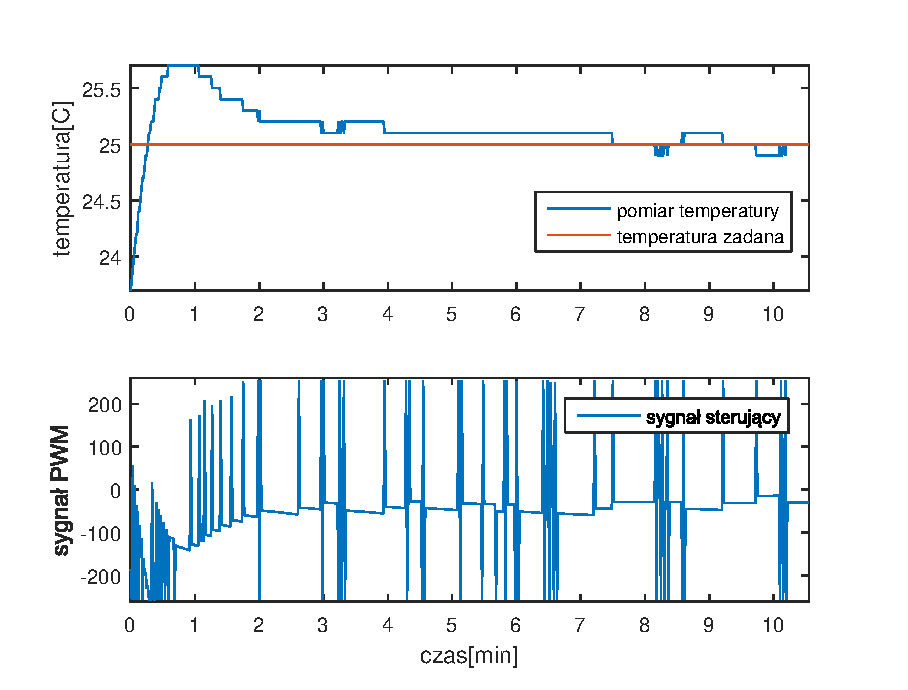
\includegraphics[scale=0.9]{pid25.eps}
	\caption{Regulacja dla $25^{\circ} C$ }
	\label{fig:pid25}
\end{figure}
\begin{figure}[H]
	\centering
	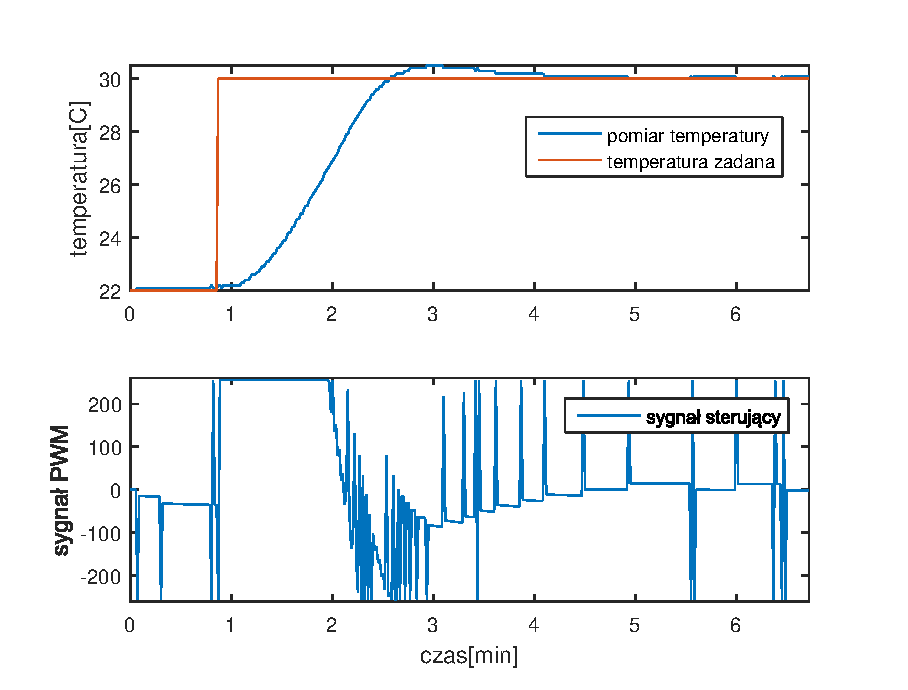
\includegraphics[scale=0.9]{pid30.eps}
	\caption{Regulacja dla $30^{\circ} C$ }
	\label{fig:pid30}
\end{figure}
\section{Aplikacja mobilna}
Podczas wykonywania pomiarów, nastawy oraz wartości zadane były przesyłane przez aplikację mobilną. W celu wygenerowania wykresów, do Arduino został podłączony komputer, nasłuchujący informacje przesyłane przez Arduino na porcie UART. Poniżej zamieszczono kilka zdjęć, wykonanych podczas regulacji temperatury za pomocą regulatora PID.
\begin{figure}[H]
	\centering
	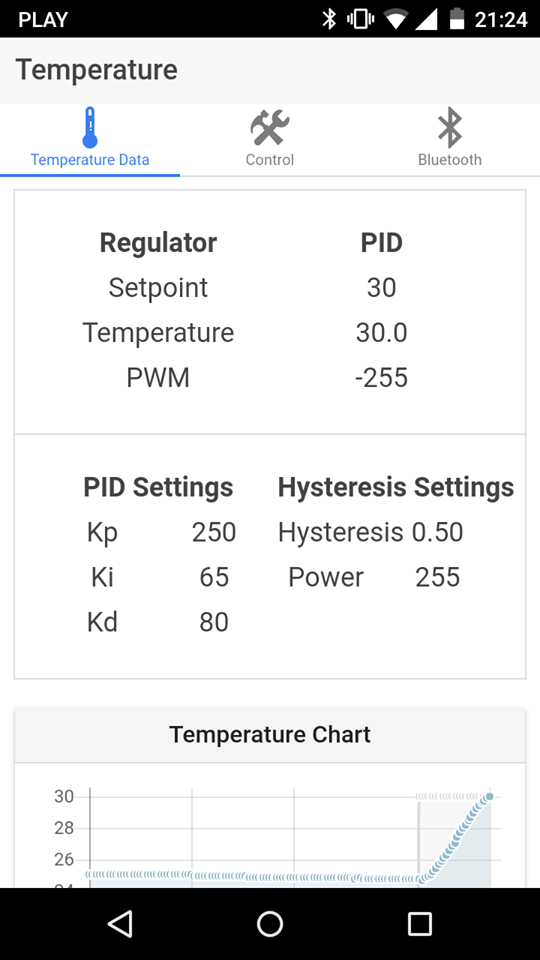
\includegraphics[scale=0.25]{testApki1.png}
	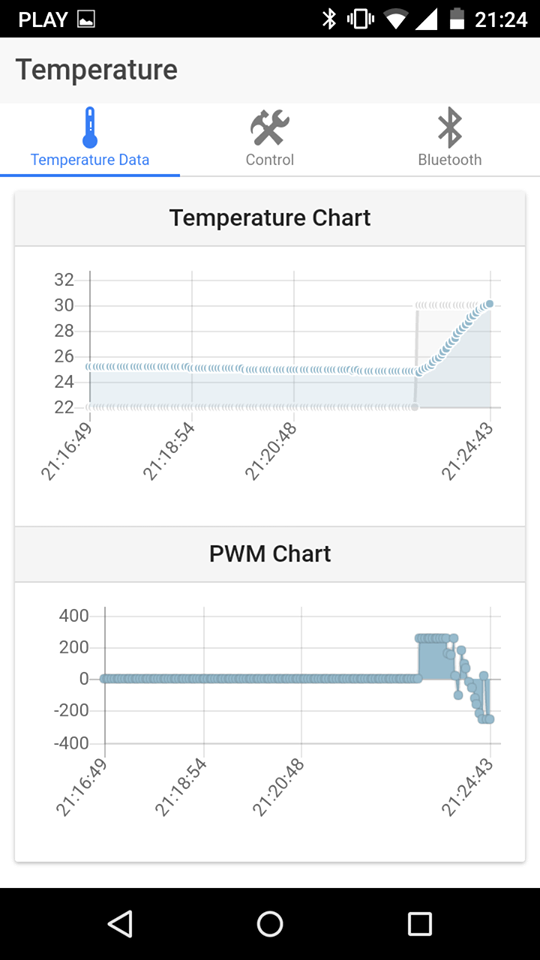
\includegraphics[scale=0.25]{testApki2.png}
	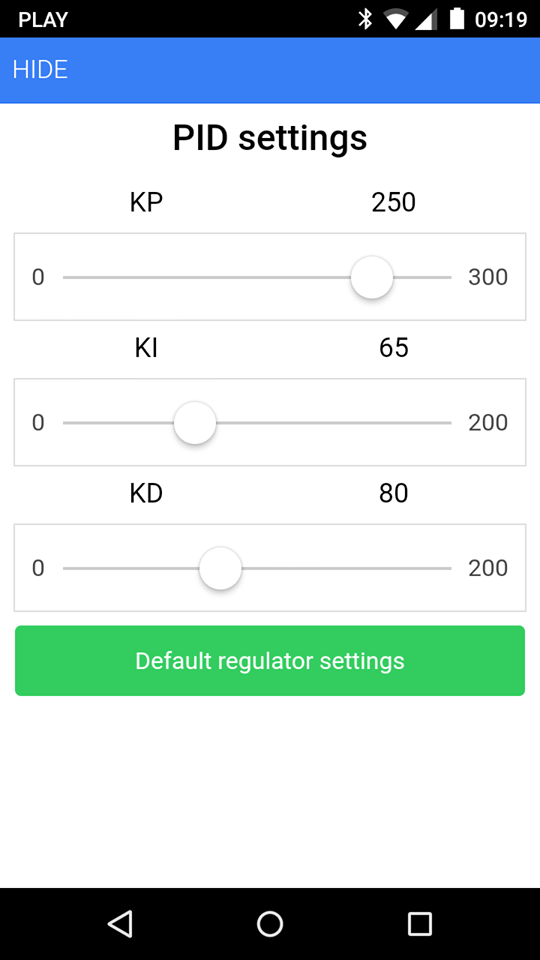
\includegraphics[scale=0.25]{apka4.png}
	\caption{Test działania aplikacji}
\end{figure}

%%%%%%%%%%%%%%%%%%%%%%%%	Podsumowanie
\chapter{Podsumowanie}
Wynikiem niniejszej pracy inżynierskiej jest skonstruowany obiekt oraz układ regulacji temperatury. Pomimo pewnych trudności napotkanych na początku budowy układu regulacji, po prawidłowym doborze radiatorów do ogniwa Peltiera, prace nad projektem nabrały szybszego tempa. Główne prace zostały zakończone na tyle szybko, że podjęto decyzję o dodaniu do pracy aplikacji mobilnej, kosztem rezygnacji z mniej interesujących elementów. Aplikacja została dostosowana do urządzeń mobilnych z oprogramowaniem Android. W celu przyspieszenia regulacji temperatury, w ostatecznej wersji obiekt został pomniejszony. Niniejsza praca pozwoliła na rozwinięcie się w obszarach zainteresowań autora oraz na poznanie nowych metod tworzenia aplikacji. Zaprojektowane oprogramowanie sterujące, dobrze radzi sobie z regulacją temperatury w wybranym zakresie. Aplikacja mobilna pozwala na przetestowanie regulatora histerezowego oraz PID, w dowolnej konfiguracji.

W przypadku przyszłych modyfikacji, warto byłoby, aby układ regulacji temperatury został oparty o płytkę STM lub AVR. Ponadto, można by pomyśleć o rozbudowaniu obiektu do postaci makiety domu jednorodzinnego lub biurowca, w którym zostałyby zainstalowane dodatkowe czujniki oraz sterowano by oświetleniem. Ciekawym rozwiązaniem byłoby wykorzystanie protokołu komunikacji ZigBee, z którego zrezygnowano podczas wykonywania projektu.


%%%%%%%%%%%%%%%%%%%%%%%%		BIBLIOGRAFIA
\addcontentsline{toc}{chapter}{Bibliografia}
%\newpage
\begin{thebibliography}{99}
\bibitem{1}
\emph{Arduino Playground},
http://playground.arduino.cc/
\bibitem{seb} ktos:
\emph{tytul},
Wydawnictwo , Poznań 2000
\end{thebibliography}

\nocite{*}
\printbibliography 


%%%%%%%%%%%%%%%%%%%%%%%%		Dodatki
\chapter*{Dodatki}
\addcontentsline{toc}{chapter}{Dodatki}
Dodatek do niniejszej pracy stanowi płyta CD zawierająca:
\begin{itemize}
\item pracę dyplomową w postaci źródłowej (LaTeX),
\item pracę dyplomową w postaci pliku pdf,
\item program napisany w Arduino IDE,
\item pliki źródłowe aplikacji mobilnej,
\item aplikację w postaci paczki dystrybucyjnej app.
\end{itemize}

\newpage
\addcontentsline{toc}{section}{Spis rysunków}	
\listoffigures

\newpage
\addcontentsline{toc}{section}{Spis tablic}	
\listoftables

%%%%%%%%%%%%%%%%%%%%%%%%

\end{document}